\documentclass[a4paper,12pt,polish,oneside,openright]{thesis}
\usepackage{listings}
\usepackage{multicol}
\usepackage{multirow}
\usepackage{chngcntr}
\usepackage{pdfpages}
\usepackage{url}
\usepackage[polish]{babel}

\counterwithout{figure}{chapter}
\counterwithout{table}{chapter}

\lstdefinestyle{line}{
	language=C,
	basicstyle=\ttfamily,
}

\lstdefinestyle{code}{
	language=C,
	basicstyle=\ttfamily\scriptsize,
	numbers=left,
	numberstyle=\tiny,
	numbersep=5pt,
	showspaces=false,
	showstringspaces=false,
	showtabs=false,
	tabsize=2,
	captionpos=t,
	breaklines=true,
	frame=single,
	breakatwhitespace=false,
}

\lstdefinestyle{coden}{
	language=C,
	basicstyle=\ttfamily\scriptsize,
	showspaces=false,
	showstringspaces=false,
	showtabs=false,
	tabsize=2,
	captionpos=t,
	breaklines=true,
	frame=single,
	breakatwhitespace=false,
}

\newcommand\code[1]{\lstinline[style=line]{#1}}
\renewcommand{\lstlistlistingname}{Spis listingów}

\autor{Patryk Kwiatkowski}
\tytul{Implementacja podstawowej biblioteki grafów w~języku C}
\tytulAng{Implementation of the basic graph library in C}
\promotor{dr inż. Ireneusz Szcześniak}
\rok{2012}
\kierunek{Informatyka}
\specjalnosc{Sieciowe Technologie Informatyczne}
\numerAlbumu{101510}
\studia{stacjonarne}
\stopien{II}

\makeatletter
\def\cleardoublepage{\clearpage\if@twoside \ifodd\c@page\else
\hbox{}
\vspace*{\fill}
\vspace{\fill}
\thispagestyle{plain}
\newpage
\if@twocolumn\hbox{}\newpage\fi\fi\fi}
\makeatother

\begin{document}

\stronaTytulowa

%TODO podziękowania

\tableofcontents

\chapter*{Cel pracy}
\addcontentsline{toc}{chapter}{Cel pracy}
Celem pracy jest stworzenie oprogramowania komputerowego umożliwiającego tworzenie aplikacji, wykorzystujących w~swym działaniu elementy matematycznej teorii grafów.
Oprogramowanie to, dalej zwane \emph{biblioteką} powinno dostarczyć interfejs programistyczny (API), pozwalający na tworzenie oraz działanie na podstawowych elementach grafów.
Biblioteka ta powinna również implementować jeden z~wybranych algorytmów teorii grafów.

Oprogramowanie to powinna poprawnie działać na systemach operacyjnych rodziny Linux, przy zachowaniu jak najmniejszych wymagań na ich zasoby pamięciowe oraz obliczeniowe.
Powinna również dostarczać mechanizm testów jednostkowych --- bazujących na dowolnej platformie testowej --- pozwalających na dalszy rozwój oprogramowania.

Spełniając powyższe wymagania, biblioteka ta powinna zostać stworzona przy użyciu języka C. Zachowując przy tym prostotę oraz przejrzystość kodu źródłowego.
Kod ten powinien być również dobrze udokumentowany, zarówno za pomocą poniższej pracy jak i~wygenerowanej automatycznie dokumentacji.

\chapter*{Wstęp}
\addcontentsline{toc}{chapter}{Wstęp}
Systemy nawigacji GPS, sieć Internet, gry komputerowe, translatory języków obcych, biologia, chemia, socjologia --- to wszystko, i~wiele innych dziedzin życia, łączy jeden wspólny element --- teoria grafów.
Kiedy rozwój informatyki pozwolił na reprezentowanie grafów za pomocą komputera, okazało się, że algorytmy na nich oparte znajdują wiele praktycznych zastosowań.
Grafy są jednymi z~najbardziej wszechobecnych modeli zarówno świata naturalnego jak i~stworzonego przez człowieka.

Oprogramowanie oparte na analizie grafów znalazło zastosowanie w~wyznaczaniu trasy pomiędzy punktami na mapie, czy najszybszej drogi ewakuacji z~kompleksu budynków.
Przedstawienie sieci komputerowych w~postaci grafów pozwoliło na stworzenie programów usprawniających przepływ pakietów w~Internecie.
Ta dziedzina matematyki jest równie przydatna w~biologii, gdzie wierzchołek może reprezentować regiony, w~których niektóre gatunki istnieją, a~krawędzie ścieżki migracji. Informacja ta jest ważna, gdyż patrząc na powstałe wzorce, można zbadać wpływ rozprzestrzeniających się chorób, pasożytów czy zmiany ruchów na inne zwierzęta.

Dzięki możliwościom jakie dają dzisiejsze komputery w~przetwarzaniu informacji, powstało wiele bibliotek obsługujących obliczenia oparte o~teorię grafów.
Rozwiązania te pojawiają się w~niemal każdym języku programowania, od \emph{C++}, przez \emph{D}, aż do \emph{Pythona} czy \emph{Matlaba}.
Tematyka teorii grafów, ze względu na szeroką gamę zastosowań oraz dużą przydatność --- zwłaszcza przy analizie, projektowaniu oraz udoskonalaniu sieci komputerowych --- została wybrana przez autora, jako temat przewodni niniejszej pracy naukowej.
Mimo istnienia dużej ilości bibliotek komputerowych implementujących zagadnienia tej tematyki, niewiele z~nich cechuje się prostotą oraz przejrzystością kodu źródłowego.
Zaś wiele z~nich zazwyczaj zużywa wiele zasobów pamięciowych, oraz działa względnie powolnie.
Potrzeba ograniczenia zużywanych zasobów, oraz stworzenia projektu prostego i~czytelnego, była główną motywacją autora do podjęcia się stworzenia ,,\emph{Implementacji podstawowej biblioteki grafów w~języku C}''.

Rozdział pierwszy niniejszej pracy zawiera wiedzę teoretyczną posiadaną, lub zebraną, przez autora pracy na potrzeby realizacji wcześniej przedstawionych celów.
W~rozdziale tym wymienia się i~opisuje pojęcia związane z~szeroko pojętą teorią grafów, kładąc szczególny nacisk na wykorzystywane później jej elementy.

Drugi rozdział pracy zawiera szczegółowy opis zaprojektowanej biblioteki.
Wyjaśnia powody wyboru konkretnych technologii do realizacji obranych celów.
W~rozdziale tym przedstawiona została budowa poszczególnych modułów, sposób przechowywania informacji oraz metody usprawniające pracę przy dalszym rozwoju biblioteki.
Zawiera on też kilka przykładów wykorzystania interfejsu użytkownika.

Ostatnia część pracy przedstawia porównanie stworzonego na cele pracy projektu, z~istniejącymi już rozwiązaniami.
Porównania te zostały przeprowadzone pod kątem ilości zużywanej pamięci, oraz czasu jaki jest potrzebny na wykonanie podstawowych funkcji tego typu biblioteki.

Dodatkowo na końcu pracy, jako załącznik, zamieszczona została automatycznie wygenerowana, anglojęzyczna dokumentacja niniejszej biblioteki.

\chapter{Wybrane zagadnienia teorii grafów}
Rozdział ten, powstał w~celu zdefiniowania oraz wyjaśnienia elementarnych pojęć związanych z~teorią grafów. Wiadomości w~nim zawarte opierają się na publikacjach \cite{graphtheory} oraz \cite{graphtheory2}, w~których można odnaleźć więcej szczegółowych informacji.
Pojęcia te będą często używane w~dalszych częściach pracy, zatem usystematyzowanie tej wiedzy jest niezwykle istotne, aby dobrze zrozumieć sens przekazywanych słów.

\begin{description}
	\item[Teoria~grafów] dział matematyki i~informatyki zajmujący się badaniem własności grafów, matematycznych struktur wykorzystywanych do modelowania relacji pomiędzy obiektami.

	\item[Graf] (ang. \emph{graph}) \emph{G}, struktura matematyczna składająca się z~niepustego zbioru skończonego \emph{V(G)}, którego elementy nazywamy wierzchołkami i~skończonego zbioru \emph{E(G)} różnych par różnych elementów zbioru \emph{V(G)}, które nazywamy krawędziami.

	\item[Wierzchołek] (ang. \emph{vertex}), inaczej węzeł, element składowy grafu, reprezentuje obiekt rzeczywisty, punkt odniesienia, dzięki czemu krawędzie między węzłami mogą reprezentować relacje. Często numerowany, może jednak posiadać etykietę (nazwę).

	\item[Krawędź] (ang. \emph{edge}) łączy ze sobą dwa wierzchołki grafu (w~szczególnym wypadku wierzchołek sam ze sobą). Może posiadać kierunek (krawędź skierowana), lub nie (krawędź nieskierowana). Często posiada wagę/koszt, czyli przypisaną liczbę, która oznaczać może odległość między węzłami.

	\item[Droga] inaczej ścieżka to trasa wyznaczana przez krawędzie, polegająca na podróżowaniu od wierzchołka do wierzchołka po łączących je krawędziach.

	\item[Sąsiad] dwa wierzchołki grafu, pomiędzy którymi istnieje krawędź.
\end{description}

Ze względu na kierunkowość krawędzi, możemy wyróżniamy trzy podstawowe rodzaje grafów:
\begin{itemize}
	\item Nieskierowane (grafy proste) --- wszystkie krawędzie grafu są nieskierowane.
	\item Skierowane (digrafy) --- wszystkie krawędzie grafu są skierowane.
	\item Mieszane --- może zawierać jednocześnie krawędzie skierowane i~nieskierowane.
\end{itemize}

Przedstawiając obrazowo powyższe definicje można posłużyć się prostym rysunkiem:
\begin{figure}[htb]
	\begin{center}
		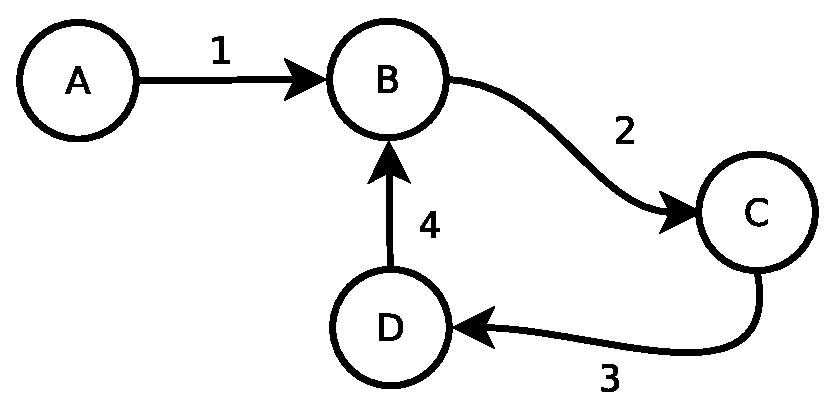
\includegraphics[width=0.5\textwidth]{gfx/small_graph.eps}
		\caption{Przykład prostego grafu skierowanego}
		\label{fig:smallgraph}
	\end{center}
\end{figure}

Punkty A, B, C oraz D znajdujące się na rysunku \ref{fig:smallgraph} nazywamy \emph{wierzchołkami}, łączące je linie \emph{krawędziami} (nieskierowanymi), zaś całość tworzy strukturę \emph{grafu} (skierowanego).
Krawędzie o~wagach 1, 2 oraz 3 tworzą \emph{drogę}, z~węzła A do węzła D. Rozpoczynając trasę z~wierzchołka D nie mamy możliwości przedostania się do węzła A.
\emph{Sąsiadem} wierzchołka B jest wierzchołek C.

Wszystkie grafy mogą być reprezentowane na wiele sposobów.
Najbardziej naturalnym i~najprostszym dla człowieka jest \emph{rysunek} grafu, jednakże jest to forma reprezentacji, której komputery nie potrafią (jeszcze) zrozumieć.
Innymi metodami zapisu mogą być:
\begin{itemize}
	\item Macierz sąsiedztwa --- macierz kwadratowa o~rozmiarze \emph{n} równym ilości wierzchołków w~grafie.
	Każdy jej element oznacza liczbę krawędzi łączącą \emph{i}-ty i~\emph{j}-ty węzeł.
	Tak zaimplementowana komputerowa struktura danych gwarantuje, że operacje sprawdzenia, czy dodania oraz usunięcia krawędzi odbywają się w stałym czasie.
	Do jej wad należy duża ilość potrzebnej pamięci – O($n^2$).

	\label{neigh_list}
	\item Lista sąsiedztwa --- dla każdego wierzchołka zapamiętywana jest lista sąsiadujących z~nim węzłów.
	Metoda ta wymaga ilości pamięci proporcjonalnej do liczby krawędzi, także przejrzenie całego zbioru krawędzi jest proporcjonalne do jego rozmiaru.
	Wadą jest tu zwiększona złożoność operacji elementarnych (np. usunięcie krawędzi).

	\item Macierz incydencji --- macierz o~wymiarach odpowiadających ilości węzłów na ilość krawędzi.
	Zawiera jedynie informacje takie, że wartość w~punkcje \{i, j\} = 1 tylko, gdy \emph{j}-ta krawędź kończy się na \emph{i}-tym wierzchołku.
\end{itemize}

Dla lepszego zrozumienia owych struktur warto ponownie przeanalizować rysunek \ref{fig:smallgraph}
oraz odpowiadające mu metody zapisu:
\begin{itemize}
	\item macierz sąsiedztwa:
	\item lista sąsiedztwa:
	\item macierz incydencji:
\end{itemize}

Informacje przytoczone w~powyższym rodziale, są podstawowymi pojęciami teorii grafów, stanowią one jedynie ułamek tej rozległej dziedziny nauki, lecz pomogą zrozumieć tematykę poruszaną przez niniejszą pracę.

\section{Algorytm Dijkstry}
\label{chap:dijkstra_theory}
Problem najkrótszej ścieżki polega na znalezieniu w~spójnym\footnote{Graf możemy nazwać spójnym wówczas, gdy dla każdej pary wierzchołków istnieje droga pomiędzy nimi.} i~ważonym\footnote{Graf możemy nazwać ważonym wówczas, gdy każda z~jego krawędzi posiada atrybut wagi/kosztu.} grafie najkrótszego połączenia pomiędzy danymi wierzchołkami.
Przez najkrótszą ścieżkę rozumiemy takie połączenie między wierzchołkami, które ma najmniejszy koszt przejścia przy czym koszt przejścia określony jest jako suma wag na krawędziach ścieżki\cite{dijkstra}.
Problem ten możemy zobrazować jako problem znalezienia najszybciej drogi dla pakietów pomiędzy dwoma routerami w~sieci.
Każde z~urządzeń trasujących reprezentowane jest wówczas przez węzeł grafu a waga krawędzi może oznaczać przepustowość łącza pomiędzy nimi (informacja przydatna dla protokołów trasowania stanu łącza, np. \emph{OSPF}\cite{ospf}).

Algorytm opracowany przez holenderskiego informatyka Edsgera Dijkstrę, służy do rozwiązywania problemu najkrótszej ścieżki.
Jest jednym z~najważniejszych algorytmów teorii grafów, wykorzystywanym m. in. właśnie w~protokole trasowania \emph{OSPF}.
Warunkiem ograniczającym jego działanie jest wymóg istnienia wyłącznie nieujemnych wag krawędzi\footnote{Algorytm Forda-Bellmana pozbawiony jest tej wady, jednakże przez to charakteryzuje się dużo większą złożonością czasową\cite{graphtheory}}.
Mając dany graf z~wyróżnionym wierzchołkiem (źródłem) algorytm znajduje odległości od niego do wszystkich pozostałych węzłów.

\begin{lstlisting}[style=code,caption=Pseudokod algorytmu Dijkstry\cite{dijkstra},label=pseudo]
for each vertex v in V[G]
	d[v] := infinity
	p[v] := undefined
end for
d[s] := 0
Q := all vertices array

while (Q is not an empty)
	u := Extract-Min(Q)
	for each edge (u,v) outgoing from u
		if (d[v] > d[u] + w(u,v))
			d[v] := d[u] + w(u,v)
			previous[v] := u
		end if
end while
\end{lstlisting}
W~algorytmie tym pamiętany jest zbiór \code{Q} wierzchołków, dla których nie obliczono jeszcze najkrótszych ścieżek, wektor \code{d} odległości od wierzchołka \code{s} (źródłowego) do \emph{i}-tego, oraz wektor poprzedników \code{p}, dzięki któremu można odtworzyć odnalezioną ścieżkę.
Początkowo (wiersze: 1 --- 6) zbiór \code{Q} zawiera wszystkie wierzchołki, wektor \code{d} jest wypełniany wartościami nieskończonymi a \code{p} niezdefiniowanymi (np. \code{NULL})
Odległość dla wierzchołka źródłowego wynosi zawsze zero.
Algorytm analizuje zawsze węzły o~najmniejszej wartości \code{d[v]}, czyli te najbliższe wierzchołkowi źródłowemu.
Zapewnia to operacja \code{Extract-Min(Q)} w~wierszu 9 listingu \ref{pseudo}, która dodatkowo usuwa pobrany element ze zbioru.

Głównym elementem algorytmu jest tzw. proces ,,relaksacji'' dla każdego wierzchołka sąsiadującego z~badanym.
Jest to sprawdzenie, czy odległość pomiędzy sąsiadem (\code{v}) badanego węzła \code{u}~a~źródłowym jest większa od sumy odległości między źródłowym a~badanym i~odległości pomiędzy badanym a~jego sąsiadem.
Jeśli tak jest, to znaczy, że algorytm znalazł ,,krótszą'' ścieżkę i~należy zaktualizować tablice dystansu \code{d} oraz poprzedników \code{p}.

Istnieje kilka odmian implementacji algorytmu Dijkstry.
Najprostsza używa tablicy do przechowywania wierzchołków ze zbioru Q.
Inne wersje algorytmu używają kolejki priorytetowej lub kopca Fibonacciego.
Przy implementacji bez użycia kopca, złożoność obliczeniowa wynosi: O($n^2$), dzięki jego zastosowaniu może spaść do O($n \cdot log_{10}(n)$)\cite{graphtheory2}.
%chapterBiblioteki w systemach Unix  Linux
%co to, po co 
%section{Statyczne}
%zalety / wady jak tworzyc
%section{Współdzielone}
%zalety /wady umiejscowienie


\chapter{Realizacja biblioteki}
Do zrealizowania postawionych w~pracy celów zaprojektowano oraz zaimplementowano bibliotekę nazwaną \emph{Simple C~Graph Library}, dalej określaną akronimowi \emph{SCGL}.
Projekt ten stworzony został w~oparciu o~język C~oraz jego bibliotekę standardową (w systemach Unix/Linux: \emph{GNU libc - glibc}).
Postanowiono również, że biblioteka będzie implementować algorytm Dijkstry --- najkrótszych ścieżek --- ze względu na jego popularność oraz istotność dla modelowania sieci komputerowych.

Wyboru tego dokonano przede wszystkim ze względu na możliwość redukcji wszelkich narzutów wynikających z~cech charakterystycznych dla języków obiektowych (dziedziczenie, polimorfizm, szablony).
Dodatkowym atutem było bardzo dobre wsparcie kompilatorów oraz szeroki wybór dostępnych narzędzi dla języka C.

Projekty takie jak ten przedstawiony w niniejszej pracy często charakteryzują się dynamicznym rozwojem, zwłaszcza w początkowych fazach tworzenia.
W~celu zapewnienia poprawności zaimplementowanych już funkcjonalności, zdecydowano się skorzystać z~mechanizmu testów jednostkowych oraz platformy \emph{DejaGNU}.

Dodatkowo biblioteka wykorzystuje program \emph{make} oraz pliki reguł \emph{Makefile} do automatyzacji procesu kompilacji.

Podczas projektowania każdego z~modułów biblioteki wykorzystano wiedzę zawartą w publikacjach (\cite{unix}, \cite{ansi}) oraz stosowano się do reguły KISS (ang. \emph{Keep It Simple, Stupid}), która traktuje o tym, że im coś jest prostsze (jako koncept, oraz jako wykonanie) tym lepiej (\cite{unix}).
\label{kiss}

\section{Budowa projektu}
Rozdział ten ma za zadanie przybliżenie czytelnikowi pomysłów projektowych biblioteki SCGL.
Zawiera on opis zastosowanej architektury oraz struktury plików.
\subsection{Diagramy klas}
Diagramy przedstawione poniżej mają na celu jedynie przekazanie informacji na temat zamysłów projektowych.
Przedstawiają one strukturę systemu (biblioteki SCGL) w~modelu obiektowym, poprzez ilustracje struktur klas i~zależności między nimi.
Ponieważ do implementacji projektu wybrano język w~pełni strukturalny (\emph{C}) nie było możliwe dokładne odwzorowanie modelu UML\footnote{UML --- (ang. \emph{Unified Modeling Language} język formalny wykorzystywany do modelowania różnego rodzaju systemów.}.

\begin{figure}[htb]
	\begin{center}
		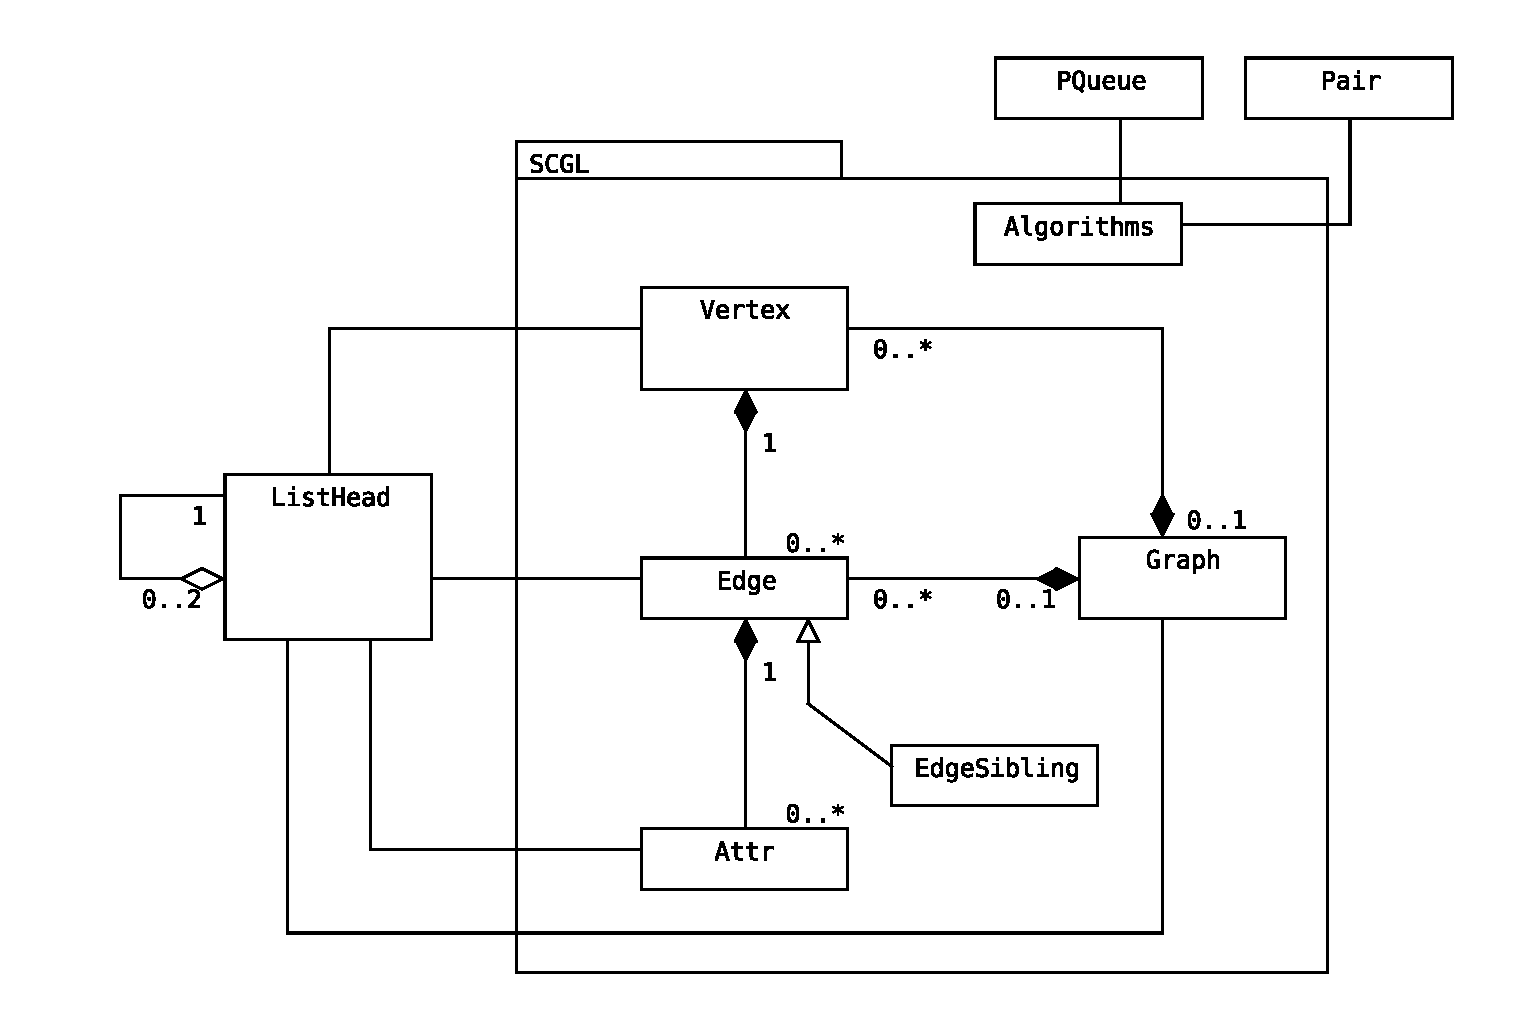
\includegraphics[width=1.00\textwidth]{gfx/class_01.eps}
		\caption{Diagram relacji pomiędzy klasami biblioteki SCGL}
	\end{center}
\end{figure}
Klasy otoczone pakietem SCGL (ramka) należą do przestrzeni nazw SCGL.
Pozostałe klasy są jedynie dodatkiem, lub kodem spoza biblioteki (nie stworzonym przez autora pracy).

\begin{description}
	\item[SCGL::Graph]
	Klasa rdzeń, najważniejsza w~bibliotece SCLG.
	Modeluje pojęcie grafu przechowując listy wierzchołków oraz krawędzi z~nimi związanych.
	Wykorzystuje do tego celu klasę \code{List\_Head}.
	Dodatkowo posiada identyfikator \code{ID}, który jest ciągiem znaków.

	Dostarcza metody pozwalające na manipulowanie zawartością swoich list węzłów i~krawędzi.
	Dodatkowo umożliwia wypisanie zawartości grafu na standardowe wyjście (lub plik), a~także wykonanie kopii grafu.
	Funkcja kopiująca, powiela wszystkie elementy grafu, również odwzorowuje powiązania pomiędzy węzłami.
	\begin{figure}[htb]
	\begin{center}
		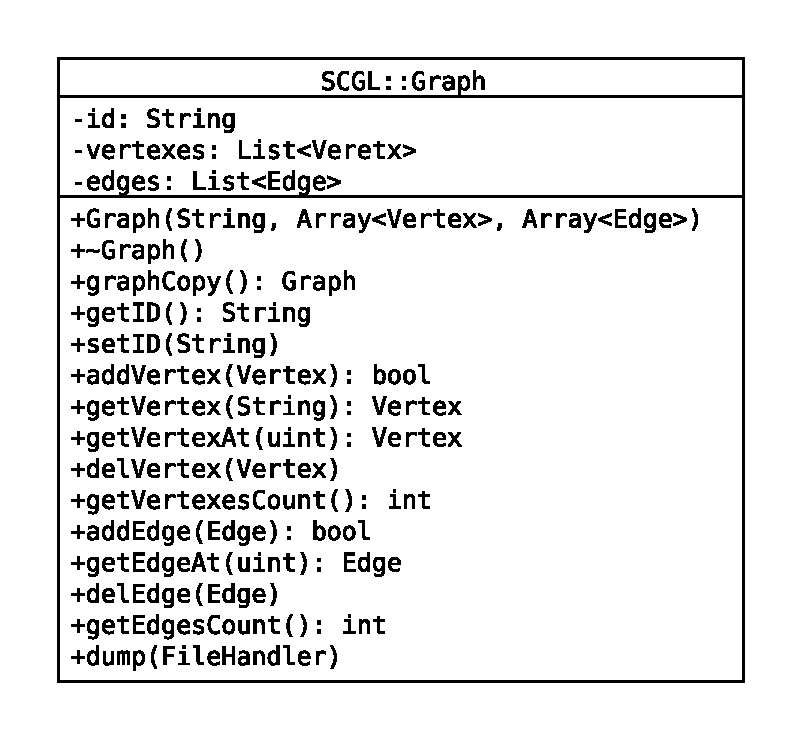
\includegraphics[width=0.60\textwidth]{gfx/class_graph.eps}
		\caption{Diagram klasy SCGL::Graph}
	\end{center}
	\end{figure}

	\item[SCGL::Edge]
	Jedna z~ważniejszych klas SCGL, reprezentuje krawędź wewnątrz grafu.
	Określana jest poprzez referencje do dwóch wierzchołków (od, do) oraz grafu, którego jest elementem składowym (tzw. ,,rodzica'').
	Dodatkowo posiada dynamiczną listę atrybutów (obiekty klasy SCGL::Attr) oraz generyczne pole koszt (zmienna typu określanego podczas kompilacji).

	SCGL::Edge przenosi również informację o~jej ,,rodzeństwie''.
	W~przypadku gdy krawędź jest nieskierowana, tworzony jest jej ,,brat'' (obiekt klasy dziedziczącej SCGL::EdgeSibling).
	Obiekt ten poprzez fakt dziedziczenia, jest klasą zawierającą dokładnie te same składowe co klasa bazowa. Jedyną różnicą jest konstruktor, który nie przyjmuje informacji o~atrybutach ponieważ nie ma potrzeby powielania tych danych.
	Wierzchołki rodzeństwa są zamienione tj. wierzchołek ,,od'' krawędzi oryginalnej, jest wierzchołkiem ,,do'' brata.

	Klasa ta dostarcza metody dostępowe do swych pól prywatnych a~także metodę która pozwala na wywołanie funkcji użytkownika na każdym z~atrybutów krawędzi.
	Dodatkowo jak wcześniej opisane klasy, umożliwia również wyprowadzenie jej zawartości na strumień.
	\begin{figure}[htb]
	\begin{center}
		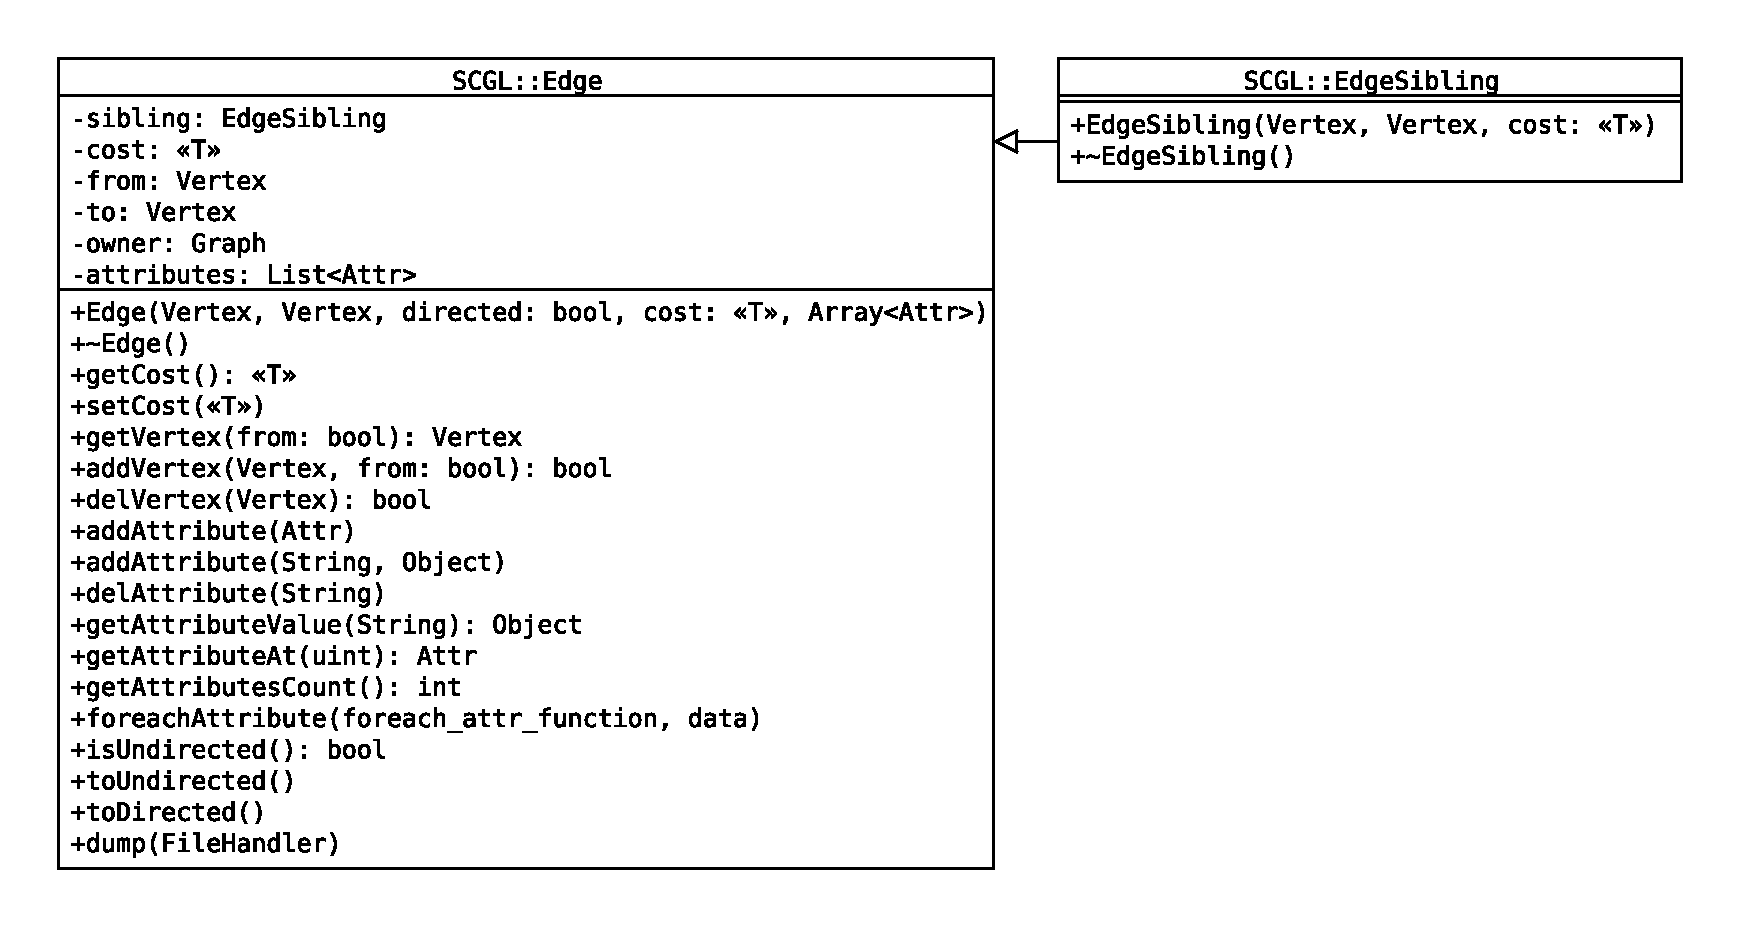
\includegraphics[width=1.00\textwidth]{gfx/class_edge.eps}
		\caption{Diagram klasy SCGL::Edge}
	\end{center}
	\end{figure}

	\item[SCGL::Vertex]
	Klasa ta reprezentuje wierzchołek grafu.
	Podobnie jak SCGL::Graph posiada identyfikator \code{ID}, który jest ciągiem znaków, oraz metody pozwalające na manipulacje nim.
	Przechowuje ona dwie listy krawędzi z~nią związanych:
	\begin{itemize}
		\item \code{in} --- wchodzących do węzła,
		\item \code{out} --- wychodzących z węzła.
	\end{itemize}
	Jednym z~pól klasy jest również referencja do grafu (jej rodzica).

	Obiekt tego typu, poza metodami dostępowymi, umożliwia wywołanie funkcji użytkownika na każdej powiązanej z~nią krawędzi, jak również wypisanie zawartości na strumień (plik lub standardowe wyjście).
	\begin{figure}[htb]
	\begin{center}
		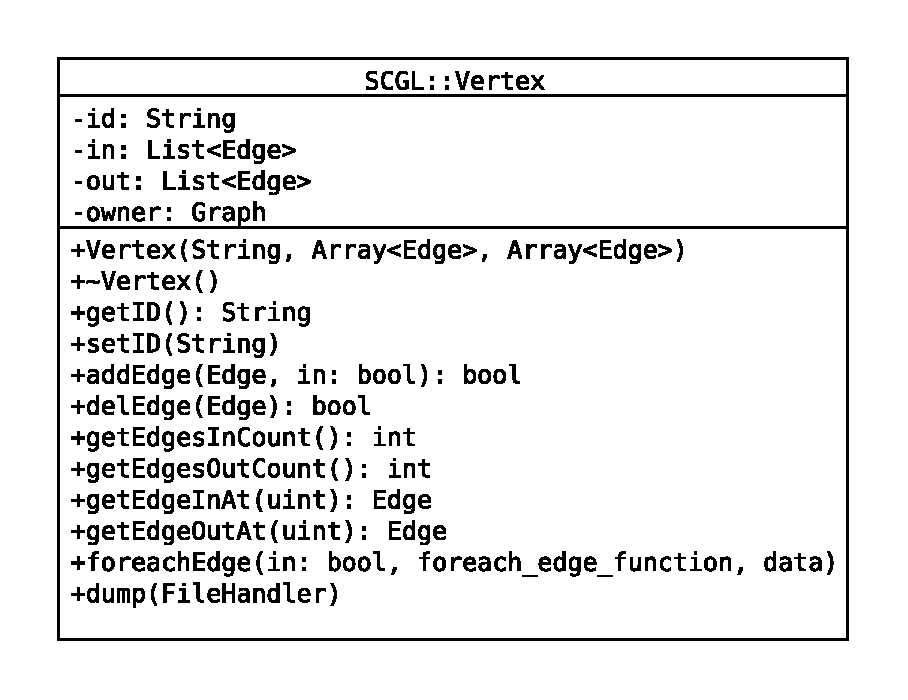
\includegraphics[width=0.55\textwidth]{gfx/class_vertex.eps}
		\caption{Diagram klasy SCGL::Vertex}
	\end{center}
	\end{figure}

	\item[SCGL::Attr]
	Klasa wykorzystywana przez obiekty SCGL::Edge, do przechowywania informacji o~jej atrybutach.
	Opisują ją dwa pola: klucz oraz wartość.
	Klucz jest ciągiem znaków, za którego unikalność odpowiedzialny jest użytkownik (nie jest to wymagane).
	Wartość zaś jest referencją do zmiennej dowolnego typu, może to być również struktura danych użytkownika.
	
	Klasa ta udostępnia jedynie konstruktor, destruktor oraz metody dostępowe.
	\begin{figure}[htb]
	\begin{center}
		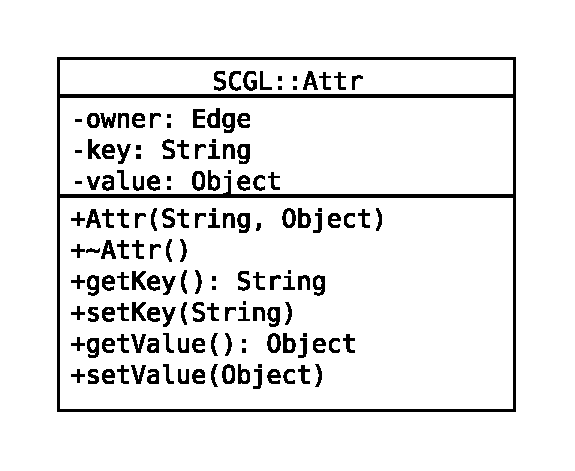
\includegraphics[width=0.4\textwidth]{gfx/class_attr.eps}
		\caption{Diagram klasy SCGL::Attr}
	\end{center}
	\end{figure}

	\item[SCGL::Algorithms]
	Jest to klasa, która dostarcza jedynie implementacje algorytmów teorii grafów.
	Aktualnie zawiera jedynie funkcję obsługującą algorytm Dijkstry, podczas działania którego wykorzystuje klasy Pair oraz PQueue.
	\begin{figure}[htb]
	\begin{center}
		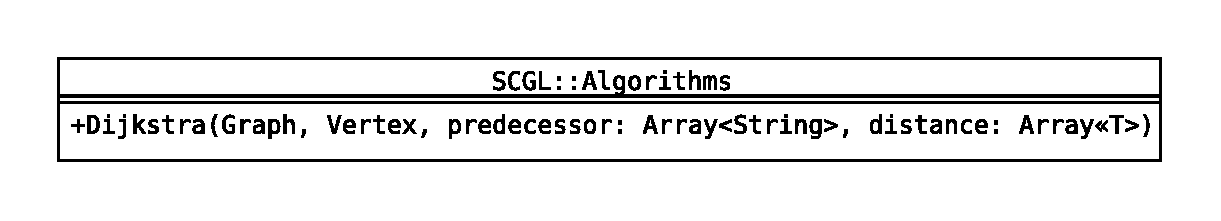
\includegraphics[width=1.0\textwidth]{gfx/class_algo.eps}
		\caption{Diagram klasy SCGL::Algorithms}
	\end{center}
	\end{figure}

	\item[ListHead]
	Klasa implementująca listę powiązaną dwukierunkową, cykliczną.
	Całkowicie ukryta przed użytkownikiem biblioteki SCGL, wykorzystywana do wewnętrznych operacji.

	\item[PQueue]
	Klasa implementująca kolejkę priorytetową opartą na kopcu.
	Również niedostępna dla użytkownika, wykorzystywana przez funkcję \code{Dijkstra} z~klasy SCGL::Algorithms.

	\item[Pair]
	Klasa implementująca kolejkę parę wartości (identyfikator, dystans)
	Wykorzystywana przez funkcję \code{Dijkstra} z~klasy SCGL::Algorithms, jako element kolejki priorytetowej.
\end{description}


\subsection{Struktura plików}
Całość projektu, kod źródłowy biblioteki, platformę testów jednostkowych, oraz dodatkowe elementy wykorzystane podczas pisania niniejszej pracy, przechowywane są przy wykorzystaniu repozytorium \emph{git}\footnote{Git --- rozproszony system kontroli wersji, stworzony przez Linusa Torvaldsa jako narzędzie wspomagające rozwój jądra Linux.}.
Owe repozytorium umieszczone jest na serwerach darmowego serwisu \url{https://github.com/}, a~jego lokalna kopia na płycie CD dołączonej do pracy (więcej na str. \pageref{chap:cd}).

Zgodnie z~dobrą praktyką programistyczną, oraz w~celu uporządkowania plików źródłowych, zastosowana została standardowa hierarchia plików.
W~katalogu głównym \emph{scgl/} (w~pliku \code{LICENSE}) znaleźć można treść licencji (dwu-klauzulowa licencja BSD) biblioteki, krótki opis projektu (\code{README}) oraz plik ułatwiający m. in. kompilację kodu \code{Makefile} (więcej na str. \pageref{chap:make}).
Kod źródłowy poszczególnych modułów SCGL znajduje się w~podkatalogu \code{src}, a~pliki definicji struktur oraz funkcje użytkownika (\emph{API}), w~podkatalogu \code{include}.

Dodatkowo wewnątrz katalogu \emph{scgl/} znajdziemy pliki stworzone przez generator dokumentacji ---  \emph{doxygen} (\code{doc/latex}).
Są to pliki tworzące dokumentację interfejsu użytkownika, przy wykorzystaniu komentarzy zawartych w~kodzie źródłowym SCGL.

Katalog \code{unit\_tests/scgl.test} zawiera definicje testów \emph{DejaGNU} oraz sam moduł wykorzystywany do testowania biblioteki.

W~folderze \code{perf\_tests} znajdują się kody źródłowe (oraz plik Makefile) testów wydajności wykorzystanych do porównania, opisanego w~rodziale \ref{chap:tests}.


\section{Szczegóły implementacji}
Do implementacji przedstawionych wcześniej diagramów, zależności oraz własności projektowych wykorzystano język C.
Jest to język strukturalny, nie posiadający cech obiektowości, brak jest tu m. in. dziedziczenia, polimorfizmu, szablonów.
Wymusiło to odseparowanie projektu biblioteki od jej ściślej implementacji.

SCGL nie posiada wewnątrz struktur pól prywatnych, wszystko jest dostępne dla użytkownika, jednak nie zalecane jest odwoływanie się do nich bezpośrednio.
W~przyszłości planowane jest jednak ukrycie owych definicji struktur przed użytkownikiem, dlatego zaleca się korzystać z~nazw alternatywnych \code{typedef}.

Język C nie posiada ,,klas'' przez co nie można za jego pomocą wywoływać metod na rzecz obiektów (jak to ma miejsce w~języku C++ np. \code{my_edge::getID()}).
Stworzono zatem specjalny system nazw (przestrzeń nazw) opisany dokładniej w~rozdziale \ref{chap:api}.

Pozostałe detale implementacyjne zostały opisane w~dalszych podrozdziałach pracy.
Wybrano elementy najistotniejsze oraz najciekawsze z~punktu działania biblioteki.

\subsection{Linux Kernel List}
\label{chap:lists}
Zjawiska modelowane przy wykorzystaniu teorii grafów, charakteryzują się zazwyczaj dużą dynamiką zmian w~czasie.
Przykładowo, w~miarę rozwoju firmy na rynku, rozwija się jej infrastruktura wewnętrzna --- struktura sieci komputerowej jest rozbudowywana o~nowe lokacje, co za tym idzie urządzenia trasujące (przedstawiane jako węzły grafu).
Fakt ciągłych zmian w~budowie grafów, narzuca niejako implementującej go bibliotece, wymaganie obsługi tego typu zdarzeń.
Musi być ona w~stanie dynamicznie zmienić rozmiary struktur, tak aby w~każdej chwili dodać (lub usunąć) wybrane elementy.

W~językach takich jak \emph{C++} najczęściej do tego celu wykorzystywane są tzw. wektory, czyli tablice o~dynamicznych rozmiarach.
Korzystając z~nich nie musimy podawać, podczas tworzenia, ilości elementów jakie będą w~nich przechowywane.
A~w~trakcie dodawania/usuwania elementów, rozmiar tablicy dostosowuje się automatycznie.

Wybrany do realizacji celów pracy język C, nie posiada wbudowanej obsługi podobnych mechanizmów wbudowanych w~standardową bibliotekę.
Istnieje co prawda możliwość rozszerzania rozmiaru tablicy (przy pomocy funkcji \code{realloc}), jednakże jest to mało wydajny mechanizm, zwłaszcza przy dużej ilości operacji dodawania/usuwania.
Innym rozwiązaniem byłyby biblioteki zewnętrze, przeznaczone dla języka C, dodające brakującą funkcjonalność.
Użycie ich może jednak wiązać się z~dodatkowymi dużymi narzutami na rozmiar biblioteki, zużywaną pamięć lub szybkość działania.
Aby zniwelować wpływ (negatywny) kodu ,,trzeciego'' na SCGL, postanowiono wykorzystać mechanizm list dowiązanych do przechowywania informacji na temat wszystkich krawędzi (ich atrybutów) oraz węzłów w~grafie.
Zasada działania jak i~implementacja tego typu list jest niezwykle prosta, a~jednocześnie nie wpływa znacząco na ilość zużywanej pamięci.

Wg klasycznego podejścia do problemu, lista jest to obiekt (struktura/klasa) zawierająca dane właściwie, oraz wskaźnik na kolejny obiekt tego samego typu.\cite{algo}
\begin{lstlisting}[style=code,caption=Idea listy powiązanej w~C]
struct list {
	struct list *prev
	struct list *next;
	void *data;
};
\end{lstlisting}
Posiadając wskaźnik, wskazujący na pierwszy element listy (\code{head}), możemy otrzymać dostęp do kolejnych danych przechowywanych wewnątrz listy poprzez wyłuskiwanie kolejnych wskaźników (\code{next}/\code{prev}).

\begin{figure}[htb]
	\begin{center}
		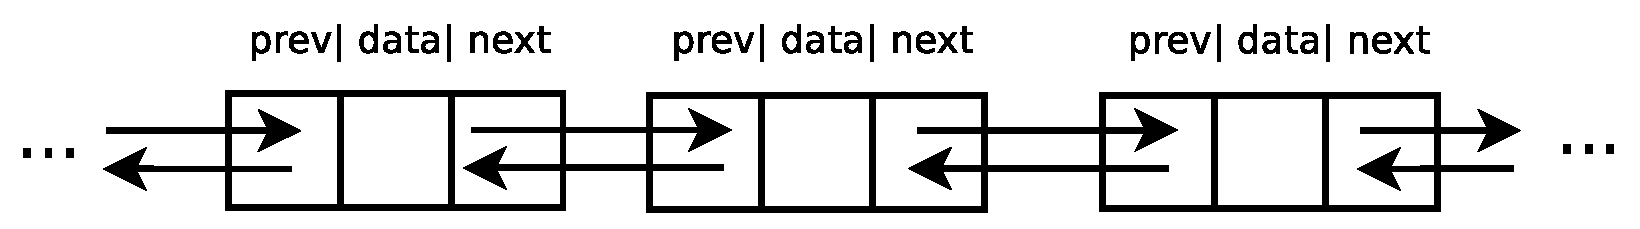
\includegraphics[width=0.80\textwidth]{gfx/linkedlist.eps}
		\caption{Kolejne elementy listy powiązanej}
	\end{center}
\end{figure}

W~niniejszej pracy postanowiono jednak skorzystać z~mechanizmu nazwanego \emph{Linux Kernel List}.
Jest to implementacja listy dowiązanej, (dwukierunkowej; cyrkulacyjnej), wykorzystywana w~jądrze (ang. \emph{kernel}) systemów operacyjnych \emph{Linux}\cite{lkl}.
Jest to jeden plik nagłówkowy (\code{*.h}) języka C.
Zawiera on definicję struktury \code{list\_head} oraz definicje i~deklaracje funkcji oraz makr preprocesora, obsługujących tą strukturę.
Linux Kernel Lists są wyjątkowe, z~powodu trochę innego podejścia do tematu.
Struktura \code{list\_head} zawiera jedynie informację (wskaźniki) na następny oraz poprzedni element listy.
Brak jest tu standardowego pola \code{data}, które przechowywałoby informacje użytkownika (tak jak jest to realizowane w~standardowej implementacji listy).
W~rozwiązaniu Linuksowym, realizacja listy daje złudzenie, że lista zawarta jest w~obiekcie który łączy (który powinien być wewnątrz niej).
Na przykład, jeśli chce się stworzyć listę powiązaną struktur \code{my\_struct}, należy zrobić to w~następujący sposób:
\begin{lstlisting}[style=code,caption=Przykład tworzenia listy powiązanej za pomocą Kernel Lined List]
struct my_struct{
	struct list_head list; /* struktura kernel list */
	int my_data;
	void *my_void;
};
\end{lstlisting}
Gdzie struktura \code{list\_head} zbudowana jest następująco:
\begin{lstlisting}[style=code]
struct list_head{
	struct list_head *prev;
	struct list_head *next;
};
\end{lstlisting}
Dołączamy strukturę listy do własnego obiektu, zamiast, obiekt do struktury listy.
Dodając kolejne elementy listy, łączymy ze sobą tak naprawdę kolejne struktury \code{list\_head}.

\begin{figure}[htb]
	\begin{center}
		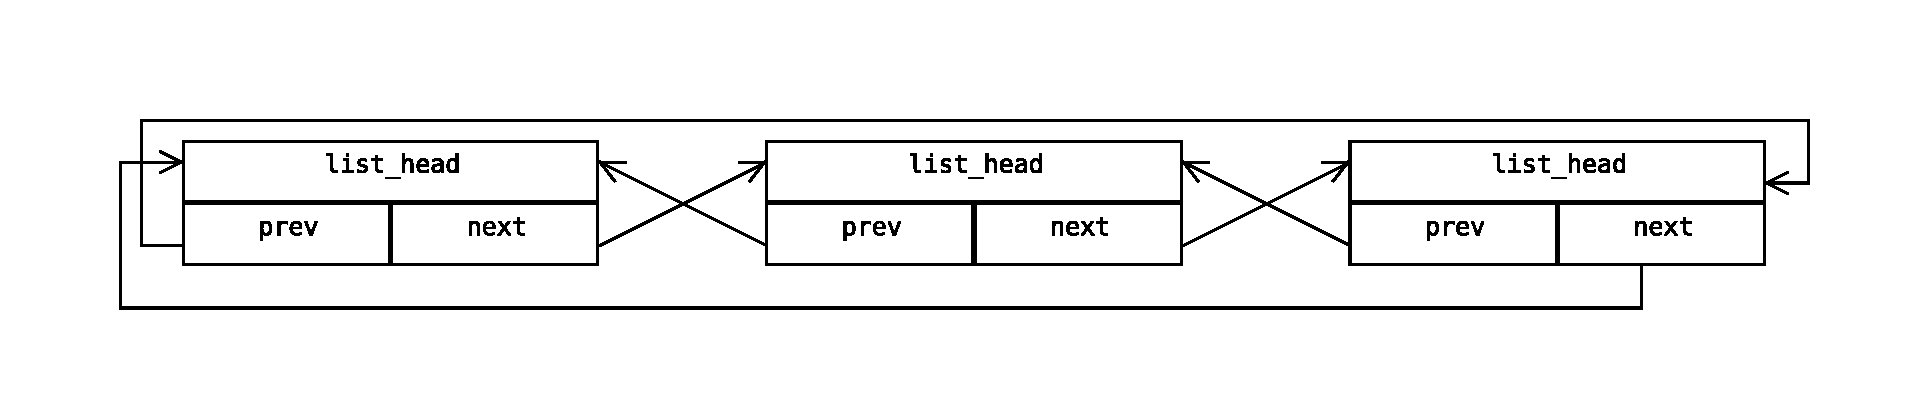
\includegraphics[width=1.05\textwidth]{gfx/list_head.eps}
		\caption{Kolejne elementy listy powiązanej w~stylu Linux Kernel List}
	\end{center}
\end{figure}

Bardzo ciekawym mechanizmem jest makro \code{container\_of} pozwalające wyznaczyć początek struktury przy pomocy jednego z~jej elementów składowych.
\begin{lstlisting}[style=coden,caption=Definicja jednego z makr jądra linuksa: {container\_of}]
#define container_of(ptr, type, member) \
	 ((type *)((char *)(ptr)-(unsigned long)(&((type *)0)->member)))
\end{lstlisting}
Otrzymując kolejno: wskaźnik na jedno z~pól struktury, typ struktury, oraz nazwę tego pola; odejmuje offset członka struktury (od jej początku) od adresu wskaźnika, dzięki czemu otrzymuje i~zwraca adres początku struktury\cite{lkl2}.
Makro to wykorzystywane jest podczas poruszania się po elementach list, do zwracania adresów struktur, podczas gdy mamy dany tylko wskaźnik na \code{list\_head\_t}.

Najważniejsze przy obcowaniu z~listami jądra Linuksa to:
\begin{itemize}
	\item Lista jest wewnątrz obiektów, które chcemy razem połączyć.
	\item Można umieścić strukturę \code{list\_head} w~każdym miejscu własnej struktury.
	\item Zmienna typu \code{list\_head} może mieć dowolną nazwę.
	\item Rozwiązanie to nie ogranicza nas do jednej listy, na cały kod źródłowy.
\end{itemize}
Ponieważ jest to mechanizm zapożyczony z jądra systemu Linux, istnieje pewność iż jest dobrze przetestowane, przenośne, szybkie oraz zajmuje niewiele pamięci.
Warto również wspomnieć, iż ten sam plik nagłówkowy, dostarcza podstaw do implementacji tablic asocjacyjnych (ang. \emph{hash list}).

Potrzebne były pewne modyfikacje, aby plik nagłówkowy \code{list.h} dostosować do zwykłego kodu, przestrzeni użytkownika (ang. \emph{userspace}):
\begin{enumerate}
	\item Została zmieniona definicja pliku nagłówkowego \code{list.h}
	\item Zostały usunięte załączone pliki nagłówkowe
	\item Zostały dodane struktury znajdujące się w~pliku \code{types.h}
	\item Wywołanie makra \code{offsetof} z~pliku \code{stddef.h}, zostało zamienione na jego treść
	\item Zmienne \code{LIST\_POISON1} oraz \code{LIST\_POISON2} zostały zastąpione przez wskaźnik na NULL --- sens pozostaje taki sam
\end{enumerate}
Dodatkowo na potrzeby biblioteki SCGL dopisana została funkcja \code{list\_count} obliczająca ilość elementów wewnątrz listy:
\begin{lstlisting}[style=code,caption=Ciało funkcji {list\_count}]
static inline unsigned int
list_count(const struct list_head *head) {
	unsigned int i = 0;
	struct list_head *j;
	list_for_each(j, head) {
		++i;
	}
	return i;
}
\end{lstlisting}

Jak już zostało wspomniane, łącząc kolejne elementy, łączymy ze sobą struktury \code{list\_head}.
Wymusza to na programiście, zmianę toku myślenia.
Chcąc przechowywać listę krawędzi wewnątrz struktury grafu, musimy w~obu tych obiektach dołączyć strukturę \code{list\_head}.
Im więcej list krawędzi chce się stworzyć, tym więcej zmiennych typu \code{list\_head} należy wpisać w~budowę obiektu.
I~tak biblioteka SCGL posiadając pięć list:
\begin{enumerate}
	\item krawędzi w grafie,
	\item węzłów w grafie,
	\item krawędzi wchodzących do węzła,
	\item krawędzi wychodzących z węzła,
	\item atrybutów krawędzi.
\end{enumerate}
Musi mieć wpisane w~struktury dziesięć, zmiennych typu \code{list\_head}.

\begin{lstlisting}[style=code,caption=Zastosowanie Linux Kernel List na przykładzie struktur biblioteki SCGL]
/** attribute object */
struct scgl_attr {
	list_head_t list;
};

/** edge object */
struct scgl_edge {
	list_head_t from_list;
	list_head_t to_list;
	list_head_t owner_list;
	list_head_t attributes;
};

/** vertex object */
struct scgl_vertex {
	list_head_t in;
	list_head_t out;
	list_head_t owner_list;
};

/** graph object */
struct scgl_graph {
	list_head_t vertexes;
	list_head_t edges;
};
\end{lstlisting}
Taka metoda przechowywania informacji przypomina nieco listy sąsiedztwa (czyt. na str. \pageref{neigh_list}), nie jest jednak dokładną ich implementacją.

Zastosowanie list powiązanych, zapożyczonych z~jądra Linuksa, pozwoliło na oszczędzenie pamięci oraz szybkości działania.
Przyśpieszyło i ułatwiło to również sam proces tworzenia biblioteki SCGL.
Nie warto tworzyć kolejnych rozwiązań od nowa, jeśli istniejące są dobrze zaimplementowane.

\subsection{Statycznie kompilowany typ zmiennej}
\label{chap:costtype}
Sporym oraz ciekawym wyzwaniem projektowym okazał się niepozorny atrybut kosztu (wagi) krawędzi, a~właściwie typ zmiennej przechowującej tą wartość.
Jak już zostało wcześniej wspomniane, element ten wykorzystywany jest przy wyborze ścieżki pomiędzy zadanymi węzłami.
Wymaganiem postawionym przed biblioteką SCGL była elastyczność typu zmiennej określającej koszt krawędzi.
Biblioteka powinna pozwalać użytkownikowi na wybór typu owego parametru według własnych preferencji, bez ingerencji w~sam kod projektu.

Problem ten dotyka tematyki paradygmatu programowania uogólnionego (generycznego, ang, \emph{generic programming}).
Pozwala on na pisanie kodu programu bez wcześniejszej znajomości typów danych, na których kod ten będzie pracował.
W~językach Java, C\#, Haskell służą do tego typy generyczne (typ ten pojawia się również w C++ dzięki zastosowaniu biblioteki \emph{boost::any}).
Zaś w~językach takich jak C++ czy D, funkcjonalność tą można zrealizować poprzez zastosowanie mechanizmu szablonów (ang. \emph{template}).
Podczas kompilacji następuje tak zwana konkretyzacja szablonu (ang. \emph{template instantiation}), podczas której kompilator na podstawie typów danych przekazanych wzorcowi generuje kod właściwy do obsługi danego typu.
Dla każdego użycia szablonu z~innym typem, generowana jest kopia odpowiednich fragmentów kodu.

Wybrany dla biblioteki SCGL język C~nie posiada żadnego z~wyżej wymienionych mechanizmów.
Aby spełnić postawione wymagania rozważano kilka możliwości projektowych, jedną z~nich było zastosowanie unii z~kilkoma podstawowymi typami zmiennych skalarnych, oraz dodatkowego pola określającego wybrany typ.
Wykorzystanie unii do tego celu, miałoby ograniczyć ilość zużytej pamięci, do największej zmiennej wewnątrz unii.
\begin{lstlisting}[style=code,caption=Koszt krawędzi jako unia]
enum cost_type {INT, DOUBLE, FLOAT};

struct scgl_edge {
   union cost {
       int i;
       double d;
       float f;
   };
   cost_type type;
};
\end{lstlisting}
Rozwiązanie to niestety wymagałoby każdorazowego sprawdzania wartości zmiennej \code{type} przed użyciem zmiennej \code{cost} (ponieważ należy wskazać którą zmienną wybieramy z~unii).
Instrukcja warunkowa \code{switch} (rozrastająca się w~miarę dodawania nowych typów do unii) negatywnie wpłynęłaby na wydajność funkcji wykorzystujących atrybut kosztu.
Alternatywnym rozwiązaniem byłoby stworzenie, dla każdego typu, funkcji posługujących się odpowiednią zmienną z~unii np:
\begin{lstlisting}[style=coden]
void scgl_dijsktra(/*...*/)
void scgl_dijkstra_int(/*...*/)
void scgl_dijkstra_float(/*...*/)
void scgl_dijkstra_double(/*...*/)
\end{lstlisting}
Zmniejszyłoby to narzut wynikający z~każdorazowego sprawdzania typu zmiennej kosztu (sprawdzanie odbywałoby się przez warper \code{scgl\_dijkstra()}, który wywoływałby odpowiednią funkcję).
Niestety rozwiązanie to jednocześnie zwiększyłoby znacznie ilość rozmiar biblioteki, dodatkowo narażając kod na błędy rodzaju copy-paste (wynikające z powielania ciała funkcji poprzez kopiowanie i~wklejanie).
Dodatkową wadą tego rozwiązania, jest fakt, iż unia zajmuje tyle miejsca co jej największa składowa. Gdyby w~jej wnętrzu znalazła się zmienna typu \code{long double} to mimo iż programista wykorzystywał by \code{cost} jako zmienną short, to pole zajmowałoby tyle bajtów ile \code{long double} na danej architekturze.

Z~powodu wyżej wymienionych cech, zdecydowano się zastosować zupełnie inne rozwiązanie.
Postanowiono stworzyć wewnątrz pliku nagłówkowego \emph{scgl\_edge.h} alternatywną nazwę (\code{typedef}), a~następnie zdefiniować wewnątrz struktury krawędzi pole będące realizacją jej kosztu w~następujący sposób:
\begin{lstlisting}[style=code,caption=Koszt krawędzi w~bibliotece SCGL]
typedef cost_type cost_type_t;

struct scgl_edge {
	cost_type_t cost;
};
\end{lstlisting}
Kod ten oczywiście nie ma prawa zadziałać, gdyż symbol \code{cost\_type} dalej pozostaje niezdefiniowany.
Odpowiedzialność za tę czynność przeniesiono do etapu kompilacji biblioteki, a~właściwie etapu translacji.
Kompilator \emph{gcc} poprzez opcję \code{-D} umożliwia definiowanie nazw, traktując je tak jakby w~kodzie pojawił się odpowiednio skonstruowany blok \code{\#define}.
\begin{lstlisting}[style=coden]
gcc -Dname=definition
gcc -Dcost_type=double
gcc -Dcost_type=int
\end{lstlisting}
Kompilując kod z~tym parametrem słowo \code{cost\_type} jest podmieniane na wybrany przez użytkownika typ, co za tym idzie zmienna \code{cost} przybiera wybrany typ.
Statyczny typ zmiennej, dobierany podczas procesu kompilacji nie powoduje dodatkowego narzutu przed jej użyciem (jak to miało miejsce w~przypadku unii), czy na rozmiar biblioteki (szablony języka C++).
Wadą jest tu jednak potrzeba rekompilacji całej biblioteki (wszystkich modułów, które korzystają ze zmiennej), za każdym razem gdy użytkownik zechce zmienić jej typ.
Jest to jednak niedogodność, którą można zaakceptować, zważywszy na możliwości, którą oferuje owe rozwiązanie.

Dodatkowym elementem wynikającym z~wybranego rozwiązania, jest potrzeba dbania o~zależności.
Wybór typu zmiennej powinien dostarczać dodatkowych informacji takich jak minimalna/maksymalna wartość zmiennej, oraz format zmiennej rozumiany przez funkcję \code{printf}.
Aby ułatwić proces budowania biblioteki, oraz zmniejszyć ewentualną możliwość popełnienia błędu przez użytkownika, postanowiono, że doborem wcześniej wymienionych wartości zajmie się plik \emph{Makefile}.
Wewnątrz tego pliku zdefiniowane są reguły budowania całej biblioteki (oraz dodatkowych elementów).
Makefile definiuje zmienną \code{COST\_TYPE}, która może przyjąć wartości odpowiadające określonemu typowi zmiennej \code{cost}.
Na podstawie wyboru użytkownika (zmiennej \code{COST\_TYPE}), Makefile dobierze odpowiednie opcję tak by biblioteka została skompilowana z~obsługą kosztu krawędzi o~wybranym typie.
W~tym celu wewnątrz pliku Makefile stworzono blok decydujący o~następującej strukturze:

\begin{lstlisting}[style=code,caption=Makefile - blok decydujący o zmiennej cost]
ifneq (,$(findstring s,$(COST_TYPE)))
	override MFLAGS:=-Dcost_type="short" -Dcost_fmt=\"%hd\" -Dcost_max=SHRT_MAX -Dcost_min=SHRT_MIN
endif
ifneq (,$(findstring us,$(COST_TYPE)))
	override MFLAGS:=-Dcost_type="unsigned short" -Dcost_fmt=\"%hd\" -Dcost_max=USHRT_MAX -Dcost_min=USHRT_MIN
endif
ifneq (,$(findstring i,$(COST_TYPE)))
	override MFLAGS:=-Dcost_type="int" -Dcost_fmt=\"%d\" -Dcost_max=INT_MAX -Dcost_min=INT_MIN
endif
ifneq (,$(findstring ui,$(COST_TYPE)))
	override MFLAGS:=-Dcost_type="unsigned int" -Dcost_fmt=\"%d\" -Dcost_max=UINT_MAX -Dcost_min=UINT_MIN
endif
ifneq (,$(findstring l,$(COST_TYPE)))
	override MFLAGS:=-Dcost_type="long" -Dcost_fmt=\"%ld\" -Dcost_max=LONG_MAX -Dcost_min=LONG_MIN
endif
ifneq (,$(findstring ul,$(COST_TYPE)))
	override MFLAGS:=-Dcost_type="unsigned long" -Dcost_fmt=\"%ld\" -Dcost_max=ULONG_MAX -Dcost_min=ULONG_MIN
endif
ifneq (,$(findstring ll,$(COST_TYPE)))
	override MFLAGS:=-Dcost_type="long long" -Dcost_fmt=\"%lld\" -Dcost_max=LLONG_MAX -Dcost_min=LLONG_MIN
endif
ifneq (,$(findstring ull,$(COST_TYPE)))
	override MFLAGS:=-Dcost_type="unsigned long long" -Dcost_fmt=\"%lld\" -Dcost_max=ULLONG_MAX -Dcost_min=ULLONG_MIN
endif
ifneq (,$(findstring f,$(COST_TYPE)))
	override MFLAGS:=-Dcost_type="float" -Dcost_fmt=\"%f\" -Dcost_max=FLT_MAX -Dcost_min=FLT_MIN
endif
ifneq (,$(findstring d,$(COST_TYPE)))
	override MFLAGS:=-Dcost_type="double" -Dcost_fmt=\"%f\" -Dcost_max=DBL_MAX -Dcost_min=DBL_MIN
endif
ifneq (,$(findstring ld,$(COST_TYPE)))
	override MFLAGS:=-Dcost_type="long double" -Dcost_fmt=\"%Lf\" -Dcost_max=LDBL_MAX -Dcost_min=LDBL_MIN
endif
\end{lstlisting}

Przedstawiony powyżej wycinek pliku Makefile porównuje zawartość zmiennej \code{COST\_TYPE} z~ustalonymi wcześniej wartościami. Na tej podstawie dobiera odpowiednie zależności, przedstawione w~tabeli \ref{tab:dep}.

\begin{table}[htb]
\caption{Zależność poszczególnych zmiennych od wartości \code{COST\_TYPE}}
\label{tab:dep}
\begin{tabular}{ | c | c | c | c | c | }
	\hline
	COST\_TYPE  & cost\_type            & cost\_fmt  & cost\_max      & cost\_min      \\
	\hline \hline
	s           & short                 & \%hd       & SHRT\_MAX      & SHRT\_MIN      \\ \hline
	us          & unsigned short        & \%hd       & USHRT\_MAX     & USHRT\_MIN     \\ \hline
	i           & int                   & \%d        & INT\_MAX       & INT\_MIN       \\ \hline
	us          & unsigned int          & \%d        & UINT\_MAX      & UINT\_MIN      \\ \hline
	l           & long                  & \%ld       & LONG\_MAX      & LONG\_MIN      \\ \hline
	ul          & unsigned long         & \%ld       & ULONG\_MAX     & ULONG\_MIN     \\ \hline
	ll          & long long             & \%lld      & LLONG\_MAX     & LLONG\_MIN     \\ \hline
	ull         & unsigned long long    & \%lld      & ULLONG\_MAX    & ULLONG\_MIN    \\ \hline
	f           & float                 & \%f        & FLT\_MAX       & FLT\_MIN       \\ \hline
	d           & double                & \%f        & DBL\_MAX       & DBL\_MIN       \\ \hline
	ld          & long double           & \%Lf       & LDBL\_MAX      & LDBL\_MIN      \\ \hline
\end{tabular}
\end{table}

Funkcja \code{findstring} wyszukuje wystąpienia pierwszego argumentu wewnątrz drugiego argumentu.
Jeśli wyszukiwanie zakończyło się sukcesem, funkcja zwraca znaleziony ciąg znaków, w~przeciwnym wypadku wynik funkcji jest równy pustemu ciągowi (dlatego sprawdzany jest warunek \code{not equal} z~pustym pierwszym argumentem).

Posługiwanie się zmienną \code{cost} odbywa się dokładnie tak jak innymi zmiennymi typu skalarnego w~języku C.
Zalecane, aczkolwiek nie wymagane, jest korzystanie z~definicji \code{cost\_max}, \code{cost\_min} oraz \code{cost\_fmt}.
Wartości \code{cost\_max} oraz \code{cost\_min} zdefiniowane są w~plikach nagłówkowych \emph{limits.h} oraz \emph{float.h}. Ich załączenie wymagane jest w~każdym pliku \code{*.c} odwołującym się do zmiennej o~typie \code{cost\_type}.

Użytkownik chcący dodać własny typ może dokonać edycji pliku Makefile.
Powinien przypisać nazwę typu do deklaracji \code{cost\_type}, jej wartość minimalną do \code{cost\_min}, maksymalną do \code{cost\_max}, oraz format dla funkcji \code{printf} do \code{cost\_fmt}.
\begin{lstlisting}[style=coden,caption=Przykład nowego typu kosztu krawędzi]
ifneq (,$(findstring nowy,$(COST_TYPE)))
	override MFLAGS:=-Dcost_type=nowy -Dcost_fmt=\"%format\" -Dcost_max=99 -Dcost_min=-99
endif
\end{lstlisting}
Należy pamiętać o~uciekaniu znaków przy definiowaniu wartości \code{cost\_fmt}.

Dzięki zaproponowanemu rozwiązaniu, biblioteka SCGL zdecydowanie zyskuje na wydajności zarówno czasowej jak i~pamięciowej, nie wprowadzając przy tym zbytniej komplikacji kodu.

\subsection{Algorytm Dijkstry}
\label{chap:dijkstra}
Do realizacji celu implementacji jednego z~algorytmów teorii grafów wybrano algorytm Dijkstry.
Wyboru tego dokonano ze względu na jego wydajność oraz istotny udział w~rozwoju sieci komputerowych, które są tematem przewodnim studiów autora pracy.

W~opisie teoretycznym algorytmu (rozdział \ref{chap:dijkstra_theory}) wspomniano, że złożoność czasowa algorytmu zależy od wykorzystanej metody przechowywania węzłów.
Aby rozwiązanie dostarczone przez bibliotekę SCGL, było możliwie jak najszybsze, zdecydowano się na użycie kolejki priorytetowej opartej na kopcu.
Złożoność algorytmu powinna wówczas wynosić O($n \cdot log_{10}{n}$).
Kolejka ta powinna priorytetować węzły na podstawie ich odległości od węzła źródłowego, oraz dostarczać operacje wyciągania elementu o~najwyższym priorytecie (najniższej odległości) oraz modyfikowania priorytetu (tzw. \emph{decrease-key}).
Postanowiono wykorzystać gotową implementację, stworzoną przez \emph{Andrei Ciobanu}\footnote{Rozwiązanie to udostępnione jest publicznie, bez licencji, a~autor kodu wyraził zgodę na użycie go w~bibliotece SCGL: \url{http://andreinc.net/2011/06/01/}}.
Kod ten zmieniono pod względem stylistycznym, tak aby pasował do reszty biblioteki SCGL, dopisano funkcję \code{pqueue_replace_data}, która realizuje operację zmiany priorytetu, oraz poprawiono kilka błędów logicznych.

Implementacja algorytmu Dijkstry napisana dla biblioteki SCGL wzoruje się na rozwiązaniu zastosowanym w~Boost::BGL\cite{bgl}.
Stosuje ona kolejkę priorytetową oraz kolorowanie węzłów, czyli operację oznaczania odwiedzonych już elementów.
\begin{lstlisting}[style=code,caption=Pseudokod implementowanego w SCGL algorytmu Dijkstry]
for each vertex u in V
	d[u] := infinity
	p[u] := u
	color[u] := WHITE
end for

color[s] := GRAY
d[s] := 0
INSERT(Q, s)
while (Q is not empty)
	u := EXTRACT-MIN(Q)
	for each vertex v in Adj[u]
		if (w(u,v) + d[u] < d[v])
			d[v] := w(u,v) + d[u]
		p[v] := u
		if (color[v] = WHITE)
			color[v] := GRAY
			INSERT(Q, v)
		else if (color[v] = GRAY)
			DECREASE-KEY(Q, v)
		end if
	end for
	color[u] := BLACK
end while
\end{lstlisting}
Jest to rozwiązanie bardzo optymalne, wykorzystanie mechanizmu kolorowania eliminuje dodatkowe (niepotrzebne) analizy mogące pojawić się w~trakcie działania algorytmu.
W~przypadku napotkania wierzchołka ,,o kolorze szarym'' wywoływana jest operacja zmiany priorytetu tego węzła w~kolejce, tak aby był on jak najniższy, wówczas będzie brany on pod uwagę w~ostatniej kolejności (w~dalszych przejściach pętli).
Niestety z~powodu zastosowania list dowiązanych w~bibliotece SCGL, realna implementacja powyższego algorytmu wymaga ciągłego obliczania jaki numer kolejny posiada określony węzeł.
Jest to operacja przechodząca po wszystkich elementach listy, do momentu odnalezienia określonego wierzchołka, co w~przypadku dużych grafów skutkować będzie znacznym spowolnieniem funkcji.
Sytuację tą poprawiłoby zastosowanie tablic asocjacyjnych (ang. \emph{hash table}), które jednoznacznie odwzorowywałby adres w~pamięci RAM z~identyfikatorem węzła.

\subsection{Testy jednostkowe - DejaGNU}
Testy jednostkowe są nieodłączną częścią każdego większego projektu programistycznego.
Jest to metoda testowania tworzonego oprogramowania poprzez weryfikowanie poprawności działania, każdego z~pojedynczych elementów (jednostek --- ang. \emph{units}) programu.
Testowany fragment poddawany jest weryfikacji, otrzymanego wyniku z~oczekiwanym (tak pozytywnym, jak i~niepozytywnym).
Testy jednostkowe pomagają weryfikować poprawność funkcji, mimo wprowadzanych zmian.
Programista wprowadzając kolejne zmiany, usprawniania, funkcjonalności, po wykonaniu testów, może mieć pewność, że jego zmiany w~kodzie nie wprowadziły kolejnych błędów.
Projektując bibliotekę SCGL, postanowiono wykorzystać właśnie tą metodę testowania, aby usprawnić przyszły jej rozwój.

Zdecydowano wykorzystać się framework DejaGNU, jako platformę do testowania.
Przeznaczeniem DejaGNU, jest stworzenie warstwy abstrakcyjnej dla wszelakich testów programistycznych\cite{dejagnu}.
Napisany został z~wykorzystaniem pakietu \emph{expect}, który jest częścią języka \emph{Tcl} (ang. \emph{Tool Command Language}).
Expect, tworzy własny terminal, który symuluje działanie użytkownika obsługującego testujący program (najczęściej konsolowy)\cite{expect}.
Pozwala on na dość elastyczną interakcję, wygodne porównywanie oraz reagowanie na wyjście docelowego programu.

Konsekwentnie stosując zasadę \emph{KISS} (czyt. str. \pageref{kiss}), również testy jednostkowe dla biblioteki SCGL zostały napisane w~sposób jasny i przejrzysty.
Platforma testowa składa się z~dwóch plików, znajdujących się w~katalogu \code{scgl/unit\_test/scgl.test}:
\begin{itemize}
	\item tests.c --- plik zawierający kody aplikacji wykorzystujących bibliotekę SCGL
	\item test.exp --- plik definiujący testy, oraz wartości oczekiwane tych testów
\end{itemize}
Program budowany przy pomocy pliku \code{tests.c} zawiera 23 podprogramy, każdy z~nich korzysta/testuje konkretną ,,jednostkę'' biblioteki SCGL.
Program ten oczekuje na wpisanie przez użytkownika: rodzaju podprogramu (wybór modułu), oraz jego numeru (wybór jednostki), a~następnie uruchamia przykładowy kod.
DejaGNU, uruchamiając kolejne testy, porównuje wartości oczekiwane, z~tymi zwróconymi przez program \code{tests.out}.
Przy pomocy wyżej opisanych plików, testowane jest:
\begin{enumerate}
	\item Tworzenie/usuwanie węzłów
	\item Ustawianie/pobieranie ID węzła
	\item Tworzenie/usuwanie krawędzi
	\item Ustawianie/pobieranie kosztu krawędzi
	\item Dodawanie/pobieranie/usuwanie węzła do/z krawędzi
	\item Dodawanie/pobieranie/usuwanie krawędzi do/z węzła
	\item Zliczanie krawędzi w węźle
	\item Wykonywanie funkcji na każdej krawędzi w węźle
	\item Tworzenie/usuwanie atrybutu krawędzi
	\item Ustawianie/pobieranie klucza atrybutu
	\item Ustawianie/pobieranie wartości atrybutu
	\item Dodawanie/pobieranie/usuwanie atrybutu do/z krawędzi
	\item Zliczanie atrybutów krawędzi
	\item Wykonywanie funkcji na każdym atrybucie
	\item Zmiana krawędzi na (nie)skierowaną
	\item Tworzenie/usuwanie grafu
	\item Ustawianie/pobieranie ID grafu
	\item Dodawanie/pobieranie/usuwanie węzła do/z grafu
	\item Dodawanie/pobieranie/usuwanie krawędzi do/z grafu
	\item Zliczanie węzłów/krawędzi w grafie
	\item Kopiowanie grafów
	\item Wykonywanie algorytmu Dijkstry na grafie skierowanym
	\item Wykonywanie algorytmu Dijkstry na grafie nieskierowanym
\end{enumerate}

\begin{lstlisting}[style=code,caption=Plik definicji testów jednostkowych platformy DejaGNU]
global TEST_APP
set test_data {
	{"vertex create/destroy"        "v 1"   "^test 0\$"}
	{"vertex set/get ID"            "v 2"   "^test_get test_set\$"}
	{"edge create/destroy"          "e 1"   "^0 1 123 123 0\$"}
	{"edge get/set cost"            "e 2"   "^123 321\$"}
	{"edge add/get/del vertex"      "e 3"   "^\\d+ 0 0 \\d+ 0 \\d+ \\d+ 0\$"}
	{"vertex add/get/del edge"      "v 3"   "^\\d+ 0 0 0 \\d+ 0\$"}
	{"vertex edges count"           "v 4"   "^0 0 1 0 1 1\$"}
	{"vertex foreach edge"          "v 5"   "^1 2 \$"}
	{"attribute create/destroy"     "a 1"   "^key value 0\$"}
	{"attribute get/set key"        "a 2"   "^key key2.\$"}
	{"attribute get/set value"      "a 3"   "^val1 val2.\$"}
	{"edge add/get/del attributes"  "e 4"   "^key1 val1 val1 0\$"}
	{"edge attributes count         "e 5"   "^1 0\$"}
	{"edge foreach attribute"       "e 6"   "^key val.\$"}
	{"edge set/get (un)directed"    "e 7"   "^0 123 1 1 \\d+ 123 1\$"}
	{"graph create/destroy"         "g 1"   "^G1 0\$"}
	{"graph get/set ID"             "g 2"   "^G1 G2.\$"}
	{"graph add/get/del vertex"     "g 3"   "^2 V2 V1 1 0 V2.\$"}
	{"graph add/get/del edge"       "g 4"   "^2 123 321 1 321 0\$"}
	{"graph vertexes/edges count"   "g 5"   "^0 0 2 2\$"}
	{"graph copy"                   "g 6"   "^0 1 1 0 1 V2 V2 0 1\$"}
	{"dijkstra directed graph       "d 1"
		"^0, 0, 0, 4, 5, 1, 1, 6, 7, 8, 9, 9, 3, 0, 1, 1, 32, 30, 15, 5, 13, 22, 31, 37, 47, 49,.\$"}
	{"dijkstra undirected graph"    "d 2"
		"^0, 0, 0, 11, 3, 1, 1, 6, 7, 11, 9, 2, 9, 0, 1, 1, 19, 21, 15, 5, 13, 22, 24, 30, 8, 29,.\$"}
}

foreach pattern $test_data {
	eval "spawn $TEST_APP [lindex $pattern 1]"
	expect {
		-re [lindex $pattern 2] { pass [lindex $pattern 0] }
		default { fail [lindex $pattern 0] }
	}
\end{lstlisting}
%TODO remove \$
Plik opisujący procedurę testowania \code{test.exp}, przechowuje tabelę \code{test_data} (linie 2--28) zawierającą kolejno: nazwę testu, argumenty przekazywane programowi oraz wartości oczekiwane (zapisane przy pomocy języka wyrażeń regularnych --- \emph{regexp}).
Część wykonawcza testu, to pętla \code{foreach} (wiersze 30-35) wywołująca kolejno testy z~tabeli \code{test_data} oraz porównująca wyniki programu z~wartościami oczekiwanymi.
Testy wywoływane są w~kolejności, która zapewnia spójność logiczną całości, np.: test dodawania atrybutu do krawędzi, jest zależy od testu tworzenia krawędzi oraz od testu tworzenia atrybutu.
Testy algorytmu Dijkstry są przeprowadzane na grafach zaprezentowanych na rysunkach \ref{fig:test_directed}, \ref{fig:test_undirected}.

Wymogiem niezbędnym do uruchomienia testów jest kompilujący się kod biblioteki SCGL, oraz posiadanie zainstalowanego w~systemie pakietu DejaGNU.
Testy uruchamiane są przez Makefile znajdujący się w~katalogu \code{scgl/}, można dokonać tego w~następujący sposób:
\begin{lstlisting}[style=coden]
make tests
\end{lstlisting}
Polecenie to wywoła kompilację pliku \code{scg/unit_tests/scgl.test/tests.c} oraz uruchomienie programu \code{runtest} (część pakietu DejaGNU) z~plikiem definicji testów: \code{test.exp}.
Jak zostało wcześniej wspomniane, testy jednostkowe są bardzo ważnym elementem oprogramowania, które będzie rozwijane.
Należy jednak pamiętać, że w~samych testach również może wkraść się błąd, należy je zatem tworzyć ze szczególną starannością.

\begin{figure}[htb]
	\begin{center}
		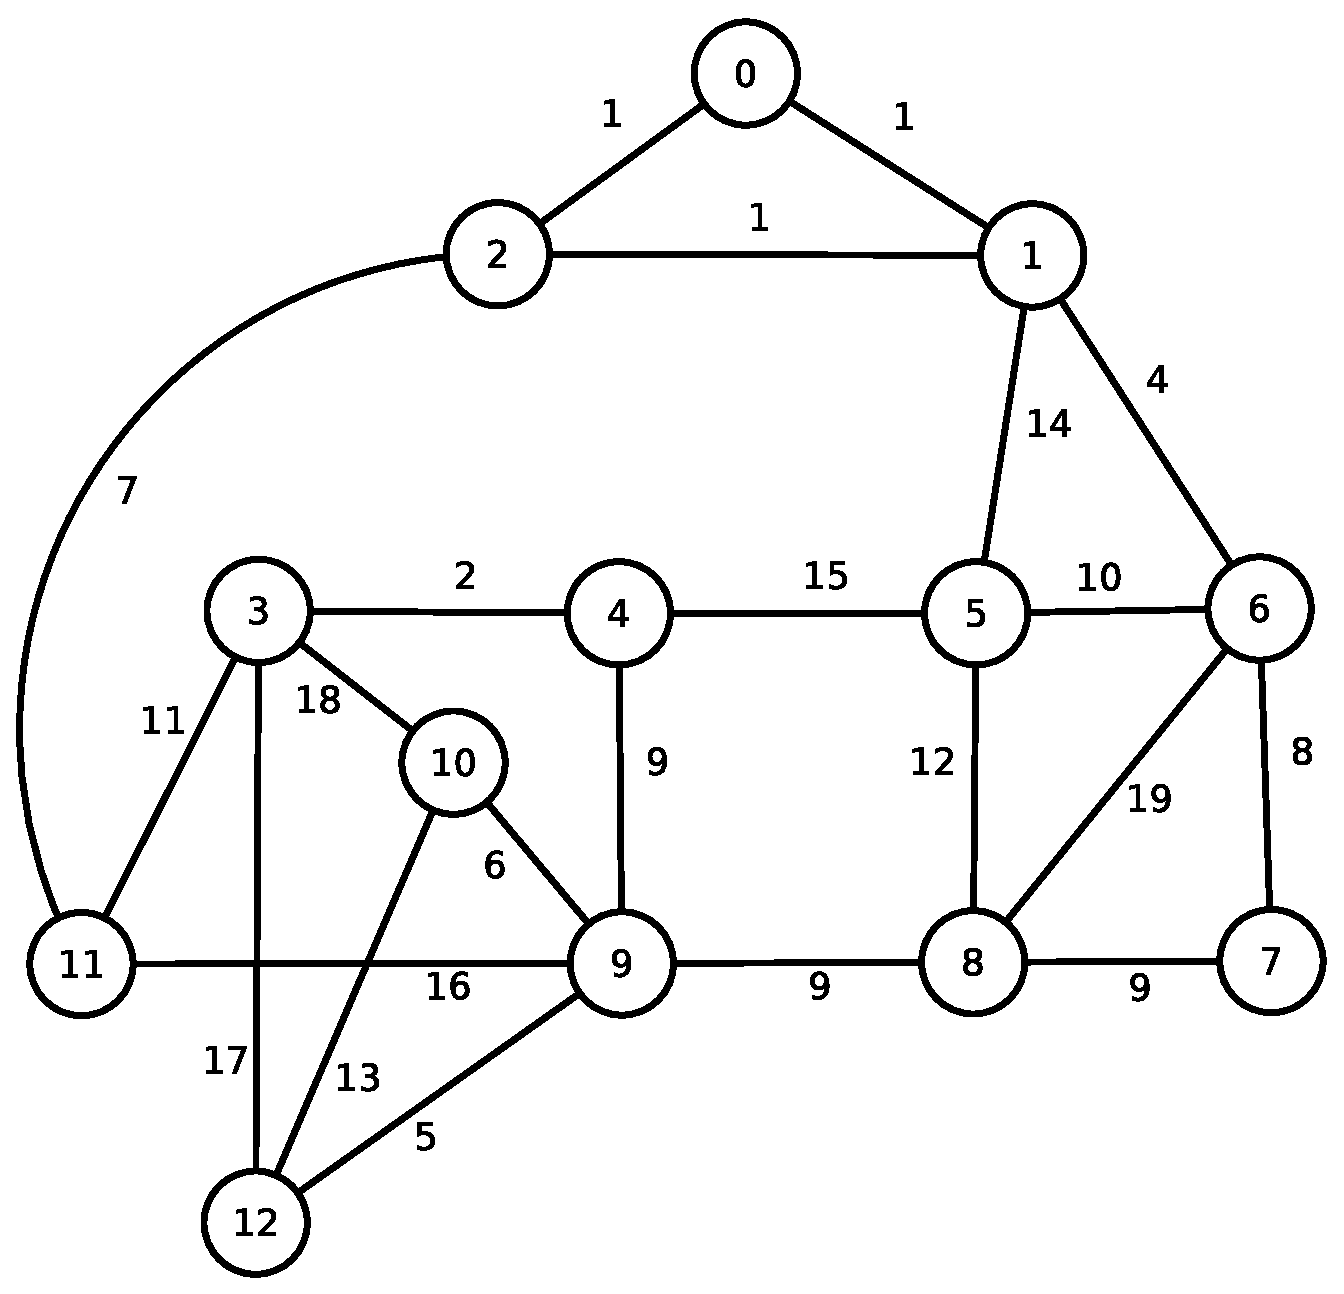
\includegraphics[width=0.65\textwidth]{gfx/test_graph_undirected.eps}
		\caption{Wykorzystywany do testów graf nieskierowany}
		\label{fig:test_undirected}
	\end{center}
\end{figure}
\begin{figure}[htb]
	\begin{center}
		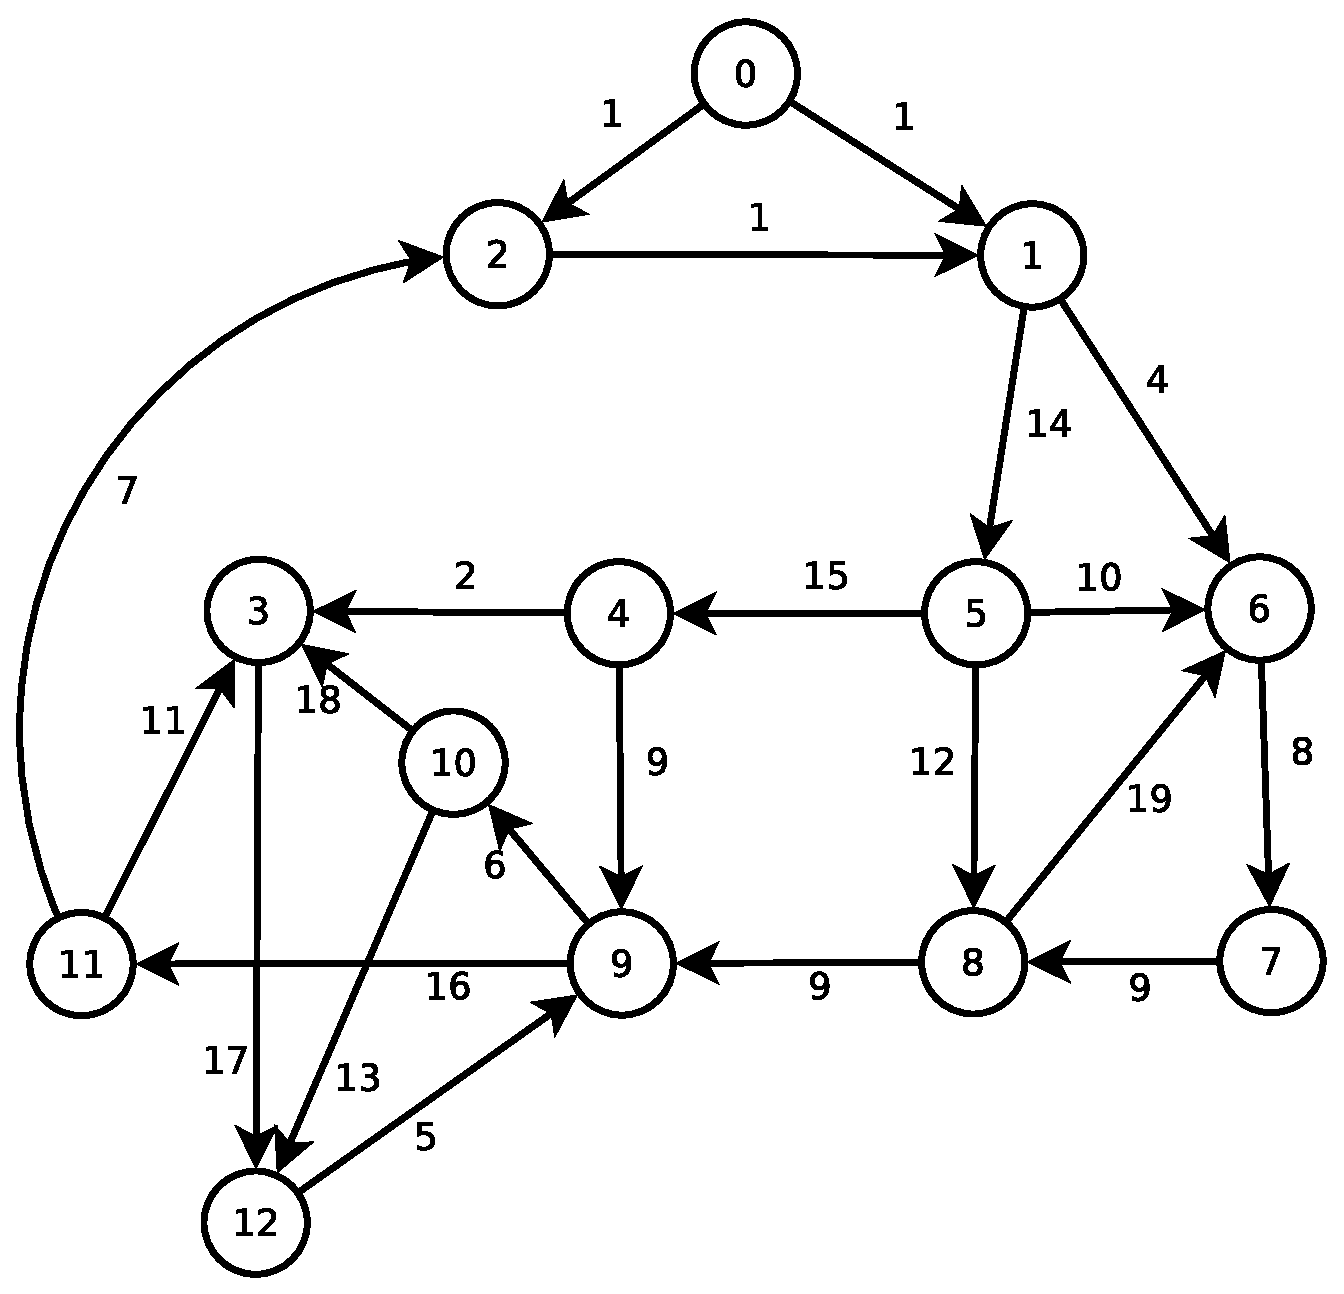
\includegraphics[width=0.65\textwidth]{gfx/test_graph_directed.eps}
		\caption{Wykorzystywany do testów graf skierowany}
		\label{fig:test_directed}
	\end{center}
\end{figure}


\section{Instrukcja użytkownika}
Niniejszy rozdział pracy ma na celu przybliżenie użytkownikowi ideologi zastosowanej dla interfejsu API oraz wyjaśnić budowę oraz sposób działania skryptów kompilujących --- Makefile.
Bardziej szczegółowe informacje na temat, każdej z~funkcji zaimplementowanej w~bibliotece SCGL dostarcza dodatek C niniejszej pracy.

\subsection{Interfejs programisty - API}
\label{chap:api}
\begin{description}
	\item[API] (ang. \emph{Application Programming Interface}), interfejs programowania aplikacji. Jego zadaniem jest dostarczenie struktur danych oraz funkcji ułatwiających manipulowanie nimi.
\end{description}
Biblioteka SCGL, jak wiele innych projektów korzystających z~języka C, wykorzystuje system prefiksów do nazewnictwa funkcji.
Wszystkie funkcje rozpoczynają się od przestrzeni nazw \code{scgl\_}, następnie występuje nazwa modułu np. \code{edge\_} i~właściwa nazwa funkcji np.:
\begin{lstlisting}[style=coden,caption=Przykłady przestrzeni nazw biblioteki SCGL,label=lst:funsuffix]
scgl_edge_add_vertex(...);
scgl_vertex_create(...);
scgl_graph_destroy(...);
\end{lstlisting}

Definicje obiektów, czyli struktury, również posiadają przedrostek \code{scgl\_}.
Użytkownik powinien jednak, korzystać z~alternatywnej definicji nazwy typu (\code{typedef}), czyli typów zakończonych literą ,,\code{t}'' np. \code{scgl\_edge\_t}:
\begin{lstlisting}[style=coden]
scgl_edge_t moja_krawedz;
scgl_graph_t *wskaznik_na_moj_graf;
\end{lstlisting}
Docelowo nazwy te powinny być wykorzystywane do ukrycia zawartości poszczególnych struktur (odpowiednik pól prywatnych klas).

Większość, jak nie wszystkie, funkcje w~SCGL jako pierwszy argument przyjmują obiekt, który będzie podlegał modyfikacjom, lub który posiada w~swojej strukturze wymagane elementy.
Argument ten jest odpowiednikiem obiektowego wskaźnika \code{this}.
Wywołanie funkcji:
\begin{lstlisting}[style=coden]
scgl_vertex_get_edges_out_count(v);
\end{lstlisting}
W~języku C++ można by zapisać w~następujący sposób:
\begin{lstlisting}[style=coden]
using namespace scgl;
/* ... */
v::get_edges_out_count();
\end{lstlisting}

\subsubsection*{Funkcje tworzące i niszczące obiekty}
Najważniejszymi funkcjami biblioteki SCGL, są oczywiście te pozwalające na stworzenie oraz zniszczenie obiektów grafowych (grafu, węzła, krawędzi).
Funkcje te, we wszystkich modułach, przyjmują te same sufiksy (końcówki nazwy), odpowiednio dla tworzenia \code{\_create} i~niszczenia \code{\_destroy}.
Przykłady tych funkcji znajdują się na listingu \ref{lst:funsuffix} w~liniach 2-3.

Podczas korzystania z~tych funkcji należy pamiętać o~pewnych elementach:
\begin{itemize}
	\item Funkcje tworzące alokują potrzebną ilość pamięci zwracając wskaźnik na początek struktury.
	\item Funkcje niszczące wymagają podania referencji do wskaźnika, dzięki temu po uwolnieniu pamięci jest on zerowany.
	\item Funkcja niszcząca krawędzie (oraz graf) wymaga podania wskaźnika do funkcji, która będzie potrafiła uwolnić pamięć dla opcjonalnych atrybutów krawędzi.
\end{itemize}

\subsubsection*{Atrybuty krawędzi}
Podstawowym atrybutem krawędzi w~bibliotece SCGL jest jej koszt (\code{cost}).
Istnieje on zawsze, dla każdej krawędzi, inicjowany jest przez użytkownika w~trakcie tworzenia obiektu.

Dodatkowo biblioteka przewiduje możliwość wykorzystywania atrybutów definiowanych przez użytkownika.
Atrybuty te reprezentowane są przez strukturę \code{scgl\_attr}.
Z~punktu widzenia użytkownika SCGL, ważne jest, że struktura ta symuluje działanie elementów tablicy asocjacyjnej.
Wartość \code{value} jest powiązana z~kluczem \code{key} (dbanie o~niepowtarzalność klucza nie jest wymagana).
Każda z~krawędzi posiada listę (więcej na str. \pageref{chap:lists}) obiektów \code{scgl\_attr}.
Dzięki temu istnieje możliwość przechowywania dowolnej ilości atrybutów w~pojedynczej krawędzi (ograniczeniem jest jedynie pamięć RAM oraz SWAP systemu).

Manipulowanie atrybutami z~poziomu krawędzi umożliwiają metody:
\begin{enumerate}
	\item \code{scgl_edge_add_attribute}
	\item \code{scgl_edge_add_attribute_object}
	\item \code{scgl_edge_del_attribute}
	\item \code{scgl_edge_get_attribute_value}
	\item \code{scgl_edge_get_attribute_at}
	\item \code{scgl_edge_get_attributes_count}
	\item \code{scgl_edge_foreach_attribute}
\end{enumerate}
Dokładny opis działania oraz zwracane wartości opisuje dokumentacja znajdująca się w~dodatku A.

Wyjaśnienie zasad programowania przy pomocy funkcji \code{scgl\_edge\_foreach\_attribute}, zostało przedstawione na stronie \pageref{sec:foreach}.

Ponieważ wartości atrybutów przetrzymywane są jako wskaźnik ogólny (\code{void*}), brak jest tu informacji na temat jej typu.
Może być to problematyczne podczas pisania funkcji niszczącej atrybuty (uwalniającej dynamicznie przydzieloną im pamięć).
Programista korzystając cały czas, z~takich samych typów wartości atrybutów nie ma powodów do zmartwień.
Chcąc jednak posiadać szereg atrybutów o~różnych typach, można skorzystać z~dwóch proponowanych, przez autora pracy, rozwiązań:
\begin{description}
	\item[enum] --- wykorzystać typ wyliczeniowy \code{enum} do przechowywania informacji o~typie wartości.
	Programista musiałby wówczas stworzyć własną strukturę, w~której przechowywałby docelową wartość atrybutu krawędzi oraz jej typ.
	\item[sufiks] --- do klucza atrybutu można dołączyć ciąg znaków, który będzie definiował typ wartości atrybutu.
	Ciąg ten może być poprzedzany znakiem ,,:'' dzięki czemu łatwiej będzie parsować wartość klucza przed użyciem wartości atrybutu.
	Można wykorzystać do tego funkcję \code{strtok} znajdującą się w~pliku nagłówkowym \code{string.h}.
\end{description}

Istnieje możliwość rozszerzenia biblioteki SCGL o~atrybuty grafów oraz węzłów.
Zrezygnowano jednak z~implementacji tych funkcjonalności ze względu na chęć zużycia jak najmniejszej ilości pamięci.
Przy projektowaniu biblioteki postanowiono, że atrybuty krawędzi są najistotniejsze i~dlatego tylko dla tego modułu zostanie dopisana możliwość manipulacji nimi.

\subsubsection*{Funkcje \code{foreach}}
\label{sec:foreach}
Każdy z~trzech modułów (graph, edge, vertex) posiada specjalną funkcję z~sufiksem \code{foreach}, jest to metoda służąca do wykonania funkcji użytkownika na kolejno wszystkich elementach (w~przypadku krawędzi będą to atrybuty, w~przypadku grafu krawędzie lub węzły).
Może ona zostać wykorzystana do dowolnego celu, np. wypisania wszystkich atrybutów na ekran, lub przetworzenia ich wartości do kosztu/wagi krawędzi.

Funkcje użytkownika zdefiniowane są w~odpowiednich plikach nagłówkowych, jednakże najczęściej przyjmują one następującą formę:
\begin{lstlisting}[style=coden,caption=Przykładowa definicja funkcji użytkownika na potrzeby funkcji \code{foreach}]
typedef void (*edge_foreach_function)(scgl_edge_t *edge, void **data);
\end{lstlisting}
Funkcje te nie zwracają żadnych zmiennych.
Jako pierwszy argument przyjmują obiekt na którym wykonane zostaną działania, jako drugi dodatkowe dane, lub wskaźnik który przechowa referencję do rezultatów.

Przykładem użycia może być funkcja zrzucająca atrybut krawędzi do strumienia:
\begin{lstlisting}[style=code,caption=Przykładowa funkcja wykorzystywana przez metodę scgl\_edge\_dump]
void edge_attr_dump(char *key, void *value, void **fp) {
	if (fp != NULL && *fp != NULL)
		fprintf((FILE*)*fp, "\t\t%s : %s \n", key, (char*)value);
}
\end{lstlisting}
Funkcja ta wywoływana będzie przez metodę \code{scgl\_edge\_dump} (zrzucanie krawędzi do strumienia)
W~tym przypadku mamy dwa argumenty określające obiekt na którym funkcja będzie operować, oraz podwójny wskaźnik na dodatkowe dane.
Dane te będą wskaźnikiem na strumień (\code{FILE}), wiedząc to, możemy wykonać rzutowanie przedstawione w~wierszu 3.
Przed wykorzystaniem tego wskaźnika należy oczywiście wcześniej sprawdzić czy nie jest on zerowy (wiersz 2).

Funkcje typu \code{foreach}, mogą mieć wiele zastosowań, jednocześnie przyśpieszając pisanie oraz upraszczając kod użytkownika.
Warto również wspomnieć, że funkcje te mogą zostać zastąpione przez wykorzystanie metod iteracyjnych \code{\_get\_at()}, które zwracają i-ty element listy oraz funkcji \code{\_get\_count}.

\subsection{Kompilacja}
\label{chap:make}
Kompilacja zarówno biblioteki jak i~testów jednostkowych oraz kodów użytkownika powinna odbywać się przy wykorzystaniu dostarczonego pliku \emph{Makefile}.
Jest to plik opisujący reguły postępowania dla programu automatyzującego proces kompilacji --- \emph{make}.

Plik Makefile, dla biblioteki SCGL znajduje się w~jej głównym katalogu \code{scgl/}.
Można wydzielić w~nim trzy sekcje logiczne:
\begin{itemize}
	\item część definiującą potrzebne zmienne, oraz pliki poddawane kompilacji
	\item część decydującą o~typie kosztu krawędzi (więcej na str. \pageref{chap:costtype})
	\item część definiującą zależności oraz przebieg procesu kompilacji
\end{itemize}
Dopisując nowy moduł do biblioteki SCGL powinniśmy dopisać jego pliki źródłowe (\code{*.c}) do zmiennej \code{SOURCES}.
Makefile automatycznie wygeneruje reguły budowy plików obiektowych (\code{*.o}) bazując na nazwie pliku źródłowego.
Pliki obiektowe linkowane (dołączane) są później do pliku biblioteki SCGL \code{libscgl.a}, który może zostać załączony do kodów źródłowych użytkownika.

Chcąc skompilować bibliotekę z~użyciem domyślnego typu kosztu krawędzi (\code{unsigned int}) wystarczy wywołać:
\begin{lstlisting}[style=coden]
make
\end{lstlisting}
Chcąc wybrać inny typ, powinno się zdefiniować wartość zmiennej \code{COST\_TYPE} wg tabeli \ref{tab:dep}:
\begin{lstlisting}[style=coden]
make COST_TYPE=d
\end{lstlisting}
Powyższe wywołanie skompiluje bibliotekę z~użyciem kosztu krawędzi jako \code{double}.

\begin{lstlisting}[style=coden]
make clean
\end{lstlisting}
Skasuje pliki cząstkowe (pliki obiektowe), wynikowe (libscgl.a) oraz te wyprodukowane przez DejaGNU.
Warto wykonywać to polecenie, jeśli wprowadzamy jakieś zmiany w~samej bibliotece SCGL.

Aby uruchomić procedurę testów jednostkowych, użytkownik powinien wywołać program \code{make} z~celem \code{tests}:
\begin{lstlisting}[style=coden]
make tests
\end{lstlisting}
Krok ten zbuduje bibliotekę SCGL (o~ile nie została wcześniej zbudowana), zbuduje program odpowiedzialny za interfejs testowy a~następnie uruchomi platformę DejaGNU.

Dodając własny cel (kod użytkownika) do pliku Makefile, użytkownik może chcieć skompilować go z~biblioteką SCGL.
Aby zrobić to poprawnie powinien skorzystać z~poniższego przykładu:
\begin{lstlisting}[style=coden]
my_app:
	@echo "Building my application"
	@$(CC) $(CFLAGS) $(MFLAGS) $(TOPDIR)my_dir/my_app.c -o $(TOPDIR)my_dir/my_app $(TOPDIR)lib/libscgl.a
\end{lstlisting}

W~projekcie znajdują się również trzy dodatkowe pliki Makefile:
\begin{enumerate}
	\item \code{scgl/doc/latex/} --- plik generujący dokumentację doxygen do pliku \code{*.pdf}
	\item \code{scgl/doc/thesis/} --- plik generujący niniejszą pracę do pliku \code{*.pdf}
	\item \code{scgl/perf_tests/} --- plik kompilujący testy wydajności, wymaga zainstalowania w~systemie bibliotek Boost::BGL oraz igraph.
\end{enumerate}


\chapter{Porównanie z istniejącymi rozwiązaniami}
\label{chap:tests}
Jak wspomniano we wstępnie niniejszej pracy, teoria grafów jest jedną z najpotrzebniejszych dziedzin matematyki w~informatyce.
Ze względu na szeroką gamę zastosowań, powstało wiele rozwiązań implementujących w~mniejszym, lub większym stopniu ową dziedzinę.
Są to biblioteki napisane w~niemal każdym języku programowania: C, C++, D, Python, Haskell, Matlab.

Jednym z~głównych celów pracy, było stworzenie oprogramowania zużywającego jak najmniej zasobów komputera, zarówno pamięciowych jak i~obliczeniowych.
Aby potwierdzić spełnienie założeń należy porównać stworzoną bibliotekę, z~innymi rozwiązaniami.
Do porównań wybrane zostały dwie najpopularniejsze biblioteki grafów:
\begin{itemize}
	\item Boost::BGL --- część ogromnej biblioteki Boost, napisanej w~języku C++
	\item igraph --- oprogramowanie napisane w~języku C
\end{itemize}

\begin{description}
\item[Boost::BGL]
Biblioteka BGL (ang. \emph{Boost Graph Library}), została stworzona przez Jeremiego Sieka oraz grupę z~uniwersytetu Notre Dame w~USA.
Wchodzi w~skład bibliotek Boost, zawiera szablony reprezentujące grafy oraz zbiór kilkudziesięciu algorytmów grafowych\cite{bgl}.
Grafy są dostarczane w postaci generycznej, dzięki czemu z wierzchołkiem, krawędzią lub całym grafem można związać obiekt lub obiekty dowolnego typu.
Szablony z biblioteki boost::graph wykorzystują kolekcje ze standardowej biblioteki szablonów (STL).

Graf w~Boost::BGL może być reprezentowany listą sąsiedztwa, a~także przez macierz sąsiedztwa albo w~specjalnej postaci skompresowanej.
W~najprostszym przypadku, gdy krawędzie są przechowywane w wektorze, identyfikatorem wierzchołka jest liczba całkowita (indeks).

\item[igraph]
\emph{igraph} jest przestronną biblioteką grafów, wspierającą aplikacje pisane w~językach takich jak: C, R, Python, czy Ruby.
Zawiera funkcje implementujące klasyczne problemy teorii grafów, takie jak minimalne drzewa rozpinające, czy algorytmy najkrótszych ścieżek.
Potrafi również generować kilkanaście rodzajów grafów, a~także eksportować je do wielu formatów obsługiwanych przez oprogramowanie graficzne\cite{igraph}.

Jest najpopularniejszą biblioteką grafów napisaną w~języku C.
\end{description}

\section{Testy porównawcze}
Porównania wcześniej wymienionych bibliotek z~biblioteką SCGL dotyczyły wydajności obliczeniowej oraz pamięciowej, tych rozwiązań.
Na potrzeby testów stworzono trzy scenariusze testowe:
\begin{enumerate}
	\item Stopnia zużycia pamięci operacyjnej --- dokładniej maksymalnego użycia sterty (ang. \emph{heap}).
	\item Szybkości tworzenia oraz usuwania obiektów.
	\item Szybkości wykonywania algorytmu Dijkstry --- obliczania najkrótszych ścieżek.
\end{enumerate}
Każdy z~nich przeprowadzony został w~dwóch wariantach:
\begin{itemize}
	\item z wykorzystaniem krawędzi skierowanych
	\item z wykorzystaniem krawędzi nieskierowanych
\end{itemize}
Pliki źródłowe testów, znajdują się w~katalogu \code{perf\_tests}.
Przedrostek, w~nazwie pliku, wskazuje na rodzaj testu, następna litera \code{d} na wariant ,,skierowany'' (\code{u} na ,,nieskierowany'') a~ostatni znak na wykorzystaną bibliotekę: \code{s} --- SCGL; \code{b} --- BGL; \code{i} --- igraph.

Wszystkie testy zostały przeprowadzone w~tych samych warunkach.
Badania wykonano na jednordzeniowym procesorze Intel Celeron M420 taktowanym 1,6GHz oraz na pamięci RAM 400MHz (5 -- 5 -- 5 -- 18 @ CL -- RCD -- RP -- RAS).
System pod którym przeprowadzono eksperymenty to GNU/Linux Arch z~jądrem w~wersji: 3.4.0-1.
Programy zostały skompilowane przy użyciu:
\begin{itemize}
	\item gcc 4.7.0 z następującymi flagami: -s -Os
	\item g++ 4.7.0 z następującymi flagami: -s -Os
\end{itemize}

Testy mające na celu porównanie użycia czasu procesora, powtarzane były w~pętli tysiąckrotnie, a~następnie uśredniane.
Skrypt odpowiadający za powtarzanie testu przedstawiony jest na poniższym listingu:
\begin{lstlisting}[style=code]
#!/bin/bash
TIMEFORMAT="%U"
sum=0
for i in {1..1000}
do
	t=$( { time $1; } 2>&1 )
	sum=$( bc <<< "scale=10; $sum + $t" )
done
avrg=$( bc <<< "scale=3; $sum / 1000" )
echo "$avrg"
\end{lstlisting}
Jak już zostało wspomniane powtarza on wykonanie polecenia (przyjmowanego jako argument skryptu) 1000 razy, sumując czas użycia procesora, zmierzony programem \emph{time} (wartości \emph{user time}).
Testy porównujące maksymalne użycie sterty, wykonane zostały przy pomocy programu \emph{valgrind}\footnote{valgrind --- jest narzędziem do debugowania pamięci, wykrywania wycieków pamięci oraz profilowania aplikacji.}.

Test mający na celu porównać poziom wykorzystania sterty przez wybrane biblioteki, polegał na stworzeniu jednego grafu, 1000 krawędzi oraz 1001 węzłów.
Żaden ze stworzonych elementów nie przechowywał dodatkowych atrybutów.
\begin{table}[htb]
\caption{Wyniki pomiaru wykorzystania sterty}
\label{tab:mem_size}
\centering
\begin{tabular}{ | c | r | r | }
	\hline
	\multirow{2}{*}{Nazwa biblioteki } & \multicolumn{2}{|c|}{Zużycie sterty w~bajtach (ilość alokacji)} \\
	\cline{2-3}
		& Graf skierowany & Graf nieskierowany \\
	\hline \hline
	SCGL    & 76~048  (2002) & 124~048 (3003) \\ \hline
	BLG     & 44~753  (2012) &  76~745 (3012) \\ \hline
	igraph  & 112~160 (0021) & 112~160 (0021) \\ \hline
\end{tabular}
\end{table}

Jak można zauważyć w~powyższej tabeli, biblioteki BGL oraz SCGL wykorzystują więcej pamięci dla grafów nieskierowanych (wszystkie krawędzie są nieskierowane), niż dla grafów w pełni skierowanych.
W~przypadku SCGL wynika to z~faktu, iż dostosowana ona jest do przetrzymywania krawędzi skierowanych.
Obiekty nieskierowane tworzone są poprzez dołączenie do krawędzi skierowanej jej odpowiednika z~zamienionymi końcami (od/do).
Aby ograniczyć zużycie pamięci, odpowiednik ten nie przechowuje informacji na temat atrybutów.
Nie jest to wymagane, gdyż krawędź ta (odpowiednik), jest niejako zawieszony w~powietrzu i~nie jest dostępny z~poziomu samego grafu.

Wyniki pomiarów, zamieszczone w~tabeli \ref{tab:mem_size}, ukazują także, że zużycie pamięci dla dostarczonego przez autora pracy rozwiązania, są dużo mniejsze niż biblioteki igraph --- w~przypadku grafów skierowanych.
Niestety nie udało się zmniejszyć zapotrzebowania, poniżej poziomu biblioteki BGL, mimo że osiągnięto porównywalną liczbę alokacji.
Program \code{valgrind} pokazał w~przypadku kodu stosującego oprogramowanie igraph, bardzo niską liczbę alokacji (21).
Może to wynikać z~faktu zastosowania w~tym rozwiązaniu niestandardowego mechanizmu przydzielania pamięci (.

Celem kolejnego z~przeprowadzonych testów, było porównanie czasu procesora, jaki zostanie zużyty do tysiąckrotnej alokacji i~uwolnienia obiektów z~poprzedniego testu (1~graf, 1000 krawędzi, 1001 węzłów).
\begin{table}[htb]
\caption{Wyniki pomiaru wykorzystania czasu procesora podczas tworzenia/niszczenia obiektów}
\label{tab:mem_speed}
\centering
\begin{tabular}{ | c | c | c | }
	\hline
	\multirow{2}{*}{Nazwa biblioteki } & \multicolumn{2}{|c|}{Wykorzystanie czasu procesora w sek.} \\
	\cline{2-3}
		& Graf skierowany & Graf nieskierowany \\
	\hline \hline
	SCGL    & 0.384 & 0.560 \\ \hline
	BLG     & 0.563 & 0.740 \\ \hline
	igraph  & 0.295 & 0.295 \\ \hline
\end{tabular}
\end{table}
Jak wynika z~powyższych rezultatów, niska ilość alokacji biblioteki igraph przekłada się na szybkość wykonywania tych operacji.
Czasy osiągane przez to oprogramowanie są niemal dwukrotnie niższe, niż w~przypadku biblioteki BGL.
Ponownie w~przypadku SCGL oraz BLG, wyniki dla grafów nieskierowanych są gorsze niż dla skierowanych.
Biblioteka SCGL osiągnęła niższe czasy tworzenia i czyszczenia pamięci niż jej odpowiednik napisany w~C++.

Ostatni test polegał na wytyczeniu najkrótszych ścieżek z~pierwszego węzła w~grafie (indeks zerowy), do wszystkich pozostałych, przy zastosowaniu algorytmu Dijkstry (więcej na str. \pageref{chap:dijkstra}).
Podobnie jak poprzednie testy, ten bazował na dwóch grafach: skierowanym oraz nieskierowanym, oba o~nieujemnych kosztach poszczególnych krawędzi, reprezentowane są przez rysunki \ref{fig:test_directed}, \ref{fig:test_undirected}.

Z~powodu niewielkich rozmiarów badanych grafów, operacja wyznaczania ścieżek została powtórzona 10000 razy.

\begin{table}[htb]
\caption{Wyniki pomiaru wykorzystania czasu procesora podczas wykonywania algorytmu Dijkstry}
\label{tab:dijkstra}
\centering
\begin{tabular}{ | c | c | c | }
	\hline
	\multirow{2}{*}{Nazwa biblioteki } & \multicolumn{2}{|c|}{Wykorzystanie czasu procesora w~sek.} \\
	\cline{2-3}
		& Graf skierowany & Graf nieskierowany \\
	\hline \hline
	SCGL    & 0.036 & 0.052 \\ \hline
	BLG     & 0.036 & 0.049 \\ \hline
	igraph  & 0.477 & 0.800 \\ \hline
\end{tabular}
\end{table}
Jak można zauważyć w~powyższej tabeli, wyniki biblioteki igraph znacząco odstają od rozwiązań SCGL oraz BGL.
Powód tego faktu pozostaje nieznany, jednakże może to wynikać ze sposobu przechowywania informacji (na temat grafu) w~pamięci.
Stworzona na potrzeby celów pracy, biblioteka SCGL, osiąga porównywalne czasy do biblioteki BGL.
Warto zauważyć, iż SCGL korzysta z~mniej wydajnych list powiązanych, co za tym idzie, musi wykonywać dodatkowe czynności w~czasie wybierania kolejnych węzłów.
Z~tego powodu, w~przypadku dużych grafów, implementacja ta będzie mniej wydajna niż BGL.
Różnica pomiędzy czasami dla grafu skierowanego i~nieskierowanego, dla biblioteki SCGL, wynika z~dodatkowej ilości obiektów (dodatkowe krawędzie symulują ,,bezkierunkowości''), które musi przeszukać algorytm.

Dodatkowym atutem biblioteki SCGL jest jej prostota.
Z~tego powodu postanowiono przeprowadzić również porównanie rozmiarów plików wynikowych z~linkowaniem statycznym (ang. \emph{static linking}).

Konsolidacja statyczna, polega na umieszczeniu plików biblioteki (pliki z~rozszerzeniem \code{*.a}) wewnątrz aplikacji użytkownika.
Dzięki temu zabiegowi, aplikacja ta uniezależniona jest od współdzielonych plików (znajdujących się najczęściej w~\code{/usr/lib/}), które mogą ulec zmianie lub zniszczeniu --- co czyni ją w~pełni przenośną (pomijając kwestie architektury komputera).
Taki tym kompilacji wykorzystuje się również często w~rozwiązaniach opartych o~systemy wbudowane (ang. \emph{embedded}), gdzie środowisko systemowe jest ograniczone, a~aplikacja użytkownika powinna być przenośna.

Testom zostały poddane aplikacje wykorzystane przy, wcześniej opisanych, testach wydajnościowych.
\begin{itemize}
	\item \code{mem\_size} --- test wykorzystania pamięci
	\item \code{mem\_speed} --- test szybkości tworzenia/usuwania obiektów
	\item \code{dijkstra} --- test szybkości działania algorytmu Dijkstry
\end{itemize}
\begin{table}[htb]
\caption{Wyniki pomiaru rozmiarów plików wykonywalnych z~zastosowaniem różnych typów konsolidacji}
\label{tab:static}
\centering
\begin{tabular}{ | c | l | r | r |}
	\hline
	\multirow{2}{*}{Nazwa biblioteki} & \multirow{2}{*}{Nazwa aplikacji} & \multicolumn{1}{|c|}{Wynik konsolidacji} & \multicolumn{1}{|c|}{Wynik konsolidacji} \\
		& & \multicolumn{1}{|c|}{statycznej w~KiB} & \multicolumn{1}{|c|}{dynamicznej w~KiB} \\
	\hline \hline
	\multirow{3}{*}{SCGL}   & \code{mem\_size}  & 736   & 3.8   \\ \cline{2-4}
							& \code{mem\_speed} & 736   & 3.8   \\ \cline{2-4}
							& \code{dijkstra}   & 742   & 4.8   \\ \hline
	\multirow{3}{*}{BGL}    & \code{mem\_size}  & 1638  & 9.2   \\ \cline{2-4}
							& \code{mem\_speed} & 1638  & 9.2   \\ \cline{2-4}
							& \code{dijkstra}   & 1740  & 21.0  \\ \hline
	\multirow{3}{*}{igraph} & \code{mem\_size}  & 884   & 3.9   \\ \cline{2-4}
							& \code{mem\_speed} & 884   & 3.9   \\ \cline{2-4}
							& \code{dijkstra}   & 1126  & 5.1   \\ \hline
\end{tabular}
\end{table}
Dla porównania zamieszczono również rozmiary aplikacji po linkowaniu dynamicznym.
Jak można zauważyć na powyższej tabeli, rozwiązanie proponowane przez autora pracy, charakteryzuje się najmniejszymi rozmiarami plików. Cecha ta może być ogromną zaletą podczas tworzenia aplikacji na wspominane systemy wbudowane.
Widać również, że fakt wykorzystania języka C++ do stworzenia biblioteki BLG znacząco wpływa na jej rozmiary (podobną zależność autor pracy zaobserwował we wszystkich, nawet najprostszych programach napisanych w~C++).

Jako ciekawostkę można dodać, że kody źródłowe oparte na bibliotece BGL, jak i~wszystkie rozwiązania oparte na języku C++, mają przeciętnie 3---4 razy dłuższe czasy kompilacji, niż ich odpowiedniki w~języku C~(zarówno dla biblioteki igraph, jak i~SCGL).


\chapter*{Podsumowanie}
\addcontentsline{toc}{chapter}{Podsumowanie}
W~ramach niniejszej pracy naukowej, według opinii jej autora, zrealizowano wszystkie postawione w~niej cele i~wymagania.

Zaimplementowano podstawową bibliotekę grafów w~języku C --- \emph{Simple C~Graph Library: SCGL}.
Biblioteka ta podzielona została na moduły zajmujące się obsługą poszczególnych elementów teorii grafów.
Zaprojektowano oraz wdrożono jednolity interfejs programisty (API), który pozwala na dodanie obsługi grafów w~aplikacjach innego użytkownika.
Dodatkowo do biblioteki została załączona pełna dokumentacja owego API, stworzona w~języku angielskim.
SCGL obsługuje również jeden z~najważniejszych algorytmów teorii grafów --- algorytm wyszukiwania najkrótszych ścieżek Dijkstry.

Praca ta nie stanowi nowego podejścia do problemu, istnieje bowiem ogromna ilość bibliotek grafowych, w~tym również te napisane w~języku C. Jednakże jest to jedna z~bardzo nielicznych (o~ile nie jedyna) prosta implementacja podstawowych elementów teorii grafów. Dzięki temu może ona stanowić przykład pozwalający zrozumieć zasady działania algorytmów grafowych.

Zaimplementowana biblioteka potrafi tworzyć, manipulować oraz usuwać zarówno grafy jak i~ich elementy składowe (wierzchołki oraz krawędzie) a~także wyznaczać najkrótsze ścieżki przy pomocy algorytmu Dijkstry.
Pozwala ona również na przechowywanie dowolnej liczby, dowolnych typów atrybutów krawędzi, a~także dostosowanie typu atrybutu kosztu krawędzi do potrzeb użytkownika (typ kompilowany statycznie).
Cechuje się przede wszystkim prostotą oraz niezbyt dużą ilością kodów źródłowych.
Dzięki czemu pozostaje czytelna, co znacznie ułatwi przyszły rozwój tego oprogramowania.
Dodatkowo załączone do pracy, na płycie CD, repozytorium programu \emph{git}, pozwoli na poznanie historii tworzenia biblioteki.

Prostota zaproponowanego rozwiązania przekłada się również na jego wydajność.
Wykorzystując grafy skierowane SCGL zużywa mniej pamięci RAM niż biblioteka igraph.
Jest ona również dużo szybsza w~przypadku tworzenia oraz usuwania obiektów od rozwiązania proponowanego przez twórców Boost::Graph.
Dodatkowo wykazała się podobnym (do BGL) czasem wykonywania algorytmu Dijkstry dla niewielkich grafów, a~dużo mniejszym do igraph.
Biblioteka SCGL cechuje się również najmniejszymi, spośród badanych rozwiązań, rozmiarami plików wykonywalnych (zarówno w~wyniku konsolidacji dynamicznej jak i~statycznej).
Dzięki temu może być stosowana w~rozwiązaniach wbudowanych (embedded) gdzie występuje potrzeba minimalizacji zużywanej pamięci masowej FLASH/EEPROM.

Pomimo faktu, że biblioteka ta została napisana z~myślą o~systemach operacyjnych rodziny Unix/Linux, z~całą pewnością może być ona przeniesiona na inne systemy operacyjne (np. firmy Microsoft).
Pewność ta wynika z~braku zależności biblioteki od jakichkolwiek specyficznych mechanizmów systemów Unix/Linux.

Stworzoną do celów pracy bibliotekę, można by w~przyszłości rozbudować realizując zaproponowane przez autora pracy pomysły:
\begin{itemize}
	\item Dodanie kolejnych algorytmów teorii grafów, np. algorytm Bellmana-Forda, lub Prima.
	\item Przyśpieszenie działania algorytmu Dijkstry poprzez zastosowanie tabel asocjacyjnych.
	\item Ukrycie przed użytkownikiem biblioteki zawartości wszystkich struktur, wymuszając korzystanie jedynie z~dostarczonego API.
	\item Dodanie mechanizmu serializacji grafów, dzięki któremu biblioteka mogłaby być wykorzystana w~aplikacjach korzystających z~MPI\footnote{MPI (ang. \emph{Message Passing Interface}, protokół komunikacyjny będący standardem przesyłania komunikatów pomiędzy procesami programów równoległych działających na jednym lub więcej komputerach.}.
\end{itemize}
W~dalszym rozwoju biblioteki może pomóc fakt istnienia szeregu testów jednostkowych, napisanych przy wykorzystaniu platformy DejaGNU. Pozwalają one zweryfikować poprawność działania istniejących już modułów/jednostek biblioteki SCGL, przez co programista może mieć pewność, że jego zmiany nie wprowadziły dodatkowych błędów.

Autor pracy zebrał oraz przyswoił wiedzę na temat podstawowych aspektów teorii grafów, oraz działania algorytmów wyszukiwania najkrótszych ścieżek.
Pogłębił również wiedzę z~tematyki programowania w~języku C.
Zapoznał się dokładniej z~technologiami wykorzystywanymi w~jądrze systemów Linux, oraz platformą testową DejaGNU.
Posiadł umiejętności z~zakresu tworzenia bibliotek zarówno statycznych jak i~dynamicznych, oraz testów jednostkowych.
Poszerzył także wiedzę o~dobrych praktykach programistycznych.

Podsumowując można stwierdzić, że zrealizowana w~ramach niniejszej pracy implementacja podstawowej biblioteki grafów, może być skutecznie wykorzystywana do modelowania zjawisk świata rzeczywistego (np. sieci komputerowych).
Może być również niezwykle użyteczna w~procesie analizy zasad działania algorytmów teorii grafów, a~także do przybliżenia technik programistycznych umożliwiających tworzenie wydajnego oprogramowania.

\chapter*{Summary}
\addcontentsline{toc}{chapter}{Summary}


\begin{thebibliography}{19}
\bibitem{graphtheory}
Ross K.A., Wright C., \emph{Matematyka dyskretna}, PWN, 2006

\bibitem{graphtheory2}
West D.B, \emph{Introduction to Graph Theory}, Prentice Hall, 1999

\bibitem{dijkstra}
Cormen, T.H., Leiserson, C.E., \emph{Introduction to Algorithms}, MIT Press, 2009

\bibitem{ospf}
Moy J.T, \emph{OSPF: Anatomy of an Internet Routing Protocol}, Addison-Wesley, 1998

\bibitem{unix}
Raymond S.E., \emph{The Art of UNIX Programming}, Addison-Wesley Professional, 2003

\bibitem{ansi}
Kernighan B.W., Ritchie D.M., \emph{Język ANSI C. Programowanie.} Helion, 2010

\bibitem{algo}
Banachowski L., \emph{Algorytmy i struktury danych}, WNT 2011

\bibitem{bgl}
Boost Graph Library: Dijkstra's Shortest Paths, \url{http://www.boost.org/doc/libs/1_49_0/libs/graph/doc/dijkstra_shortest_paths.html}, stan na dzień 15.03.2012

\bibitem{lkl}
Linux Kernel Linked List Explained, \url{http://isis.poly.edu/kulesh/stuff/src/klist/}, stan na dzień 25.02.2012

\bibitem{lkl2}
FAQ/LinkedLists, \url{http://kernelnewbies.org/FAQ/LinkedLists}, stan na dzień 26.02.2012

\bibitem{dejagnu}
Doar M.B., \emph{Practical Development Environments}, O'Reilly Media, 2005

\bibitem{expect}
Libes D., \emph{Exploring Expect}, O'Reilly Media, 2010

\bibitem{igraph}
The igraph library for complex network research, \url{http://igraph.sourceforge.net/documentation.html}, stan na dzień 01.12.2011

\end{thebibliography}



\chapter*{Dodatek A. Dokumentacja}
\addcontentsline{toc}{chapter}{Dodatek A. Dokumentacja}

\chapter*{Dodatek B. Oświadczenie}
\addcontentsline{toc}{chapter}{Dodatek B. Oświadczenie}
\newlength{\oldparskip}
\setlength{\oldparskip}{\parskip}
\setlength{\parindent}{0pt}.
\setlength{\parskip}{0.3cm}

Imię i nazwisko: \emph{Patryk Kwiatkowski} \hfill Częstochowa, dn. \emph{\today} \\
Nr albumu: \emph{101510} \\
Kierunek: \emph{Informatyka} \\
Wydział: \emph{Wydział Inżynierii Mechanicznej i~Informatyki} \\

\vfill
Politechnika Częstochowska
\vfill
\begin{flushright}
\textbf{Szanowny Pan (i) Dziekan} \hspace*{1cm}
\end{flushright}
\vfill
\begin{center}
\textbf{\textsc{\large Oświadczenie}}
\end{center}
\vfill

Pod rygorem odpowiedzialności karnej oświadczam, że złożona przez mnie praca dyplomowa pt. \emph{,,Implementacja podstawowej biblioteki grafów w~języku C''} jest moim samodzielnym opracowaniem.

Jednocześnie oświadczam, że praca w~całości lub we fragmentach nie została dotychczas przedłożona w~żadnej szkole.

Niezależnie od art.239 Prawo o~szkolnictwie wyższym wyrażam zgodę na nieodpłatne wykorzystanie przez Politechnikę Częstochowską całości lub fragmentów w/w pracy w~publikacjach Politechniki Częstochowskiej.

\vfill

\begin{center}
	\begin{minipage}{0.7\textwidth}
		\begin{flushright}
		\begin{minipage}{0.4\textwidth}
			\begin{center}
			\dotfill\\
			podpis
			\end{center}
		\end{minipage}
		\end{flushright}
	\end{minipage}
\end{center}

\setlength{\parskip}{\oldparskip}

\chapter*{Dodatek C. Opis zawartości płyty CD}
\addcontentsline{toc}{chapter}{Dodatek C. Opis zawartości płyty CD}
\label{chap:cd}
\begin{lstlisting}[basicstyle={\small},caption={Struktura plików zamieszczonych na płycie CD}]
.
|-- praca/
|   |-- gfx
|   |-- url
|   |-- praca.lyx
|   |-- praca.pdf
|   |-- praca.tex
|   `-- praca.txt
`-- program/
    |-- dotNetFx40_Full_x86_x64.exe
        |-- bin/
            `-- src/
\end{lstlisting}

%Obja¶nienie:
%\begin{description}
%	\item [{praca/gfx/}] katalog zawieraj±cy grafiki wykorzystane w~powy¿szej
%pracy (wymagane do kompilacji pliku {*}.lyx oraz {*}.tex).

%	\item [{praca/url/}] kopia niektórych stron internetowych za³±czonych w~bibliografii.

%	\item [{praca/praca.lyx}] pierwotne ¼ród³o pracy; pozosta³e formaty s±
%wynikiem generowania.

%	\item [{program/dotNetFx40\_Full\_x86\_x64.exe}] instalator pakietu .NET 
%Framework 4.0, wymaganego do uruchomienia aplikacji.

%	\item [{program/bin/}] zawiera skompilowane, binarne, wersje programów
%opisanych w~powy¿szej pracy. Umieszczone one s± odpowiedno w~katalogach
%myTorrentClient oraz myTorrentServer. Za³±czone s± tu równie¿ wymagane
%pliki konfiguracyjne.

%	\item [{program/src/}] zawiera kod ¼ród³owy programów opisanych w~powy¿szej
%pracy, s± to projekty programu ,,Microsoft Visual C\# 2008 Express
%Edition''. Umieszczone one s± odpowiedno w~katalogach myTorrentClient
%oraz myTorrentServer.
%\end{description}

\listoffigures
\listoftables
\lstlistoflistings

\end{document}
